\documentclass[a4paper,12pt]{article}

\usepackage[utf8]{inputenc}
\usepackage[spanish]{babel}
\usepackage{amsmath}
\usepackage{amsfonts}
\usepackage{amssymb}
\usepackage{multirow}
\usepackage{blindtext}
\usepackage{enumitem}
%\usepackage{makeidx}
\usepackage{graphicx}
\usepackage{fancyhdr}
\usepackage{hyperref}
\usepackage{float}
\usepackage{color}
\usepackage{afterpage}
\usepackage{blindtext}
\definecolor{azulUC3M}{RGB}{0,0,102}
\definecolor{gray97}{gray}{.97}
\definecolor{gray75}{gray}{.75}
\definecolor{gray45}{gray}{.45}
\usepackage{listings}
\usepackage{parskip}
\usepackage{afterpage}
\usepackage{amssymb,amsfonts,latexsym,cancel}
\usepackage{float}
\usepackage{subfigure}
\lstset{ frame=Ltb,
     framerule=0pt,
     aboveskip=0.5cm,
     framextopmargin=3pt,
     framexbottommargin=3pt,
     framexleftmargin=0.4cm,
     framesep=0pt,
     rulesep=.4pt,
     backgroundcolor=\color{gray97},
     rulesepcolor=\color{black},
     %
     stringstyle=\ttfamily,
     showstringspaces = false,
     basicstyle=\small\ttfamily,
     commentstyle=\color{gray45},
     keywordstyle=\bfseries,
     %
     numbers=left,
     numbersep=15pt,
     numberstyle=\tiny,
     numberfirstline = false,
     breaklines=true,
   }
 
% minimizar fragmentado de listados
\lstnewenvironment{listing}[1][]
   {\lstset{#1}\pagebreak[0]}{\pagebreak[0]}
 
\lstdefinestyle{consola}
   {basicstyle=\scriptsize\bf\ttfamily,
    backgroundcolor=\color{gray75},
   }
 
\lstdefinestyle{C}
   {language=C,
   }
\usepackage[top=2cm]{geometry}
\pretolerance=2000
\tolerance=3000
\usepackage{verbatim} % comentarios
\renewcommand{\thefigure}{\thesection.\arabic{figure}}%renombra las figuras por capítulos y secciones
\usepackage{chngcntr}
\counterwithin{figure}{section}%estas tres últimas líneas para poner el número de la figura como sección.númeroimagen
%%\renewcommand\thefigure{\getCurrentSectionNumber-\arabic{figure}}
\counterwithin{table}{section}
\usepackage[nottoc]{tocbibind}
\usepackage{glossaries} %para acrónimos
\makeglossaries
\usepackage{afterpage} %para páginas en blanco
\usepackage{colortbl} %Para colores en las tablas
\usepackage{multirow,array}%para las tablas
%\usepackage[table,xcdraw]{xcolor}
\usepackage{ulem}%para que cuando se utilice el comando \emph{•} la palabra entre llaves esté subrayada. si lo quitamos la palabra estría en cursiva
\usepackage{eurosym} % para el euro
\renewcommand{\theequation}{\thesection.\arabic{equation}}
\counterwithin{equation}{section}
\usepackage{cite}
\usepackage{hyperref}

\begin{document}

\begin{titlepage}
\begin{sffamily}
\color{azulUC3M}
\begin{center}
%\vspace*{-1cm}
\begin{figure}[htb]
\begin{center}
\vspace*{0.6cm}

\includegraphics[width=15cm]{imagenes/Portada_Logo.png}
\vspace*{1.3cm}
\end{center}
\end{figure}
\begin{LARGE}
Grado en Ingeniería Electrónica Industrial y Automática\\%completar el nombre del grado
2017/2018 \\%indicar el curso académico
\vspace*{2cm}
\textsl{Trabajo Fin de Grado}\\
\end{LARGE}

\begin{huge}
%%\textbf{Estudio de estabilidad del robot humanoide TEO} \\
\textbf{Calibración de los sistemas electromecánicos para habilitar el control de estabilidad del robot humanoide TEO} \\
\rule{80mm}{0.1mm}\\
\vspace*{1cm}
Aitor González Martínez de la Casa %Separar cada autor con \\ 
\end{huge}

\vspace*{1cm}
\begin{Large}
Tutor\\
Juan Miguel García Haro\\
Leganés, Septiembre de 2018\\
\end{Large}
\end{center}
\vspace*{1cm}
\color{black}

\includegraphics[scale=0.65]{imagenes/creativecommons.png}\\
\emph{[Incluir en el caso de interés en su publicación en el archivo abierto]}\\
Esta obra se encuentra sujeta a la licencia Creative Commons \textbf{Reconocimiento - No Comercial - Sin Obra Derivada}

\end{sffamily}
\end{titlepage}

\newpage
$\ $
\thispagestyle{empty} %para que no se numere esta página


\pagestyle{fancy}
\fancyhead{} % Clear all header fields
\setlength\headheight{21.2pt}
\lhead{\hspace*{-0.3cm}\raisebox{-0.3\height}{
\includegraphics[scale=1]{imagenes/Interior_Logo.png}}}
\rhead{\color{azulUC3M}{\thepage}} %Poner encabezado

\renewcommand{\tablename}{\textbf{Tabla}} %para poner la palabra en mayúsucula
\renewcommand{\figurename}{\textbf{Figura}} % para poner la palabra en mayúscula
\renewcommand{\listtablename}{Índice de tablas} 

\section*{Agradecimientos}
\addcontentsline{toc}{section}{Agradecimientos}

Agradezco a mis padres todo el apoyo que me han proporcionado durante toda mi carrera, a mi hermano por estar siempre a mi lado y en general a toda mi familia. Espero que se sientan orgullosos.

A mis amigos, por brindarme tantos y tantos momentos de diversión y apoyarme en los momentos más duros.

Agradecer a mis compañeros, a los que considero también como amigos, tanto de grado como de laboratorio, el haberme hecho más amena mi trayectoria en la universidad.

A mi tutor el doctor Santiago Martínez de la Casa por haberme guiado a lo largo de todo el proyecto, al igual que al profesor Juan Miguel García Haro, que ha estado en todo momento cuando he necesitado ayuda.

Y por último, este proyecto está dedicado especialmente a mi abuelo, fallecido tristemente hace un año (se que estará orgulloso esté donde esté), y a mi abuela, por haberme cuidado durante todos estos años de universidad.

\afterpage{\null\newpage}
\newpage


\begin{abstract}

En el presente documento se va realizar el estudio de la estabilidad de robots humanoides utilizando los métodos de péndulo invertido y Cart-table para calcular el Punto de Momento Cero (ZMP). Todos los experimentos han sido realizados con el robot humanoide TEO (Task Environment Operator) del grupo de investigación RoboticsLab, en el departamento de Ingeniería de Sistemas y Automática de la Universidad Carlos III de Madrid.
\setlength{\parskip}{5mm}

Los datos para realizar dicho estudio se obtenían de los sensores de fuerza-par situados en los tobillos, para el modelo de péndulo invertido, y la Unidad de Medida Inercial (IMU) situada en el centro del robot, para el modelo Cart-table, mediante datos de aceleraciones lineales. Para realizar los experimentos los programas utilizados fueron QtCreator, que es un IDE (entorno de desarrollo integrado) multiplataforma para programar en C++, y Python, que es un lenguaje de programación interpretado cuyo objetivo es simplificar el código del programa.

Dicho proyecto consiste en someter al robot a diferentes inclinaciones para ajustar su posición de equilibrio haciendo uso de los modelos anteriormente descritos, utilizando para ello un filtro paso bajo para reducir el ruido de las medidas, y un controlador PID, que compara el estado actual con el deseado y ofrece una salida para el ZMP o punto de equilibrio del robot que se ajuste al que debería tener en la realidad.

\end{abstract}

\tableofcontents

\afterpage{\null\newpage}
\newpage

\listoffigures

\afterpage{\null\newpage}
\newpage

\listoftables

\afterpage{\null\newpage}
\newpage

\setlength{\parskip}{5mm}
\section{Introducción}

En los últimos años, la evolución en el campo de la industria ha sido tan grande que ha llegado al punto que se ha hecho necesario el desarrollo de robots para poder realizar las tareas de manera más eficaz, eficiente y segura. Estos robots pueden tener diferente apariencia y función según el ámbito al que se apliquen, desde robots industriales hasta robots para las tareas domésticas. En el campo industrial los robots pueden ser más simples ya que el entorno es principalmente estático, las tareas a desarrollar son repetitivas y automáticas, y apenas hay interacción humana. 

Pero no todos los entornos reúnen las condiciones ideales de ser estáticos y repetitivos. Por esta razón surgió la necesidad de crear robots que fueran capaces de trabajar en entornos dinámicos siendo capaces de desarrollar tareas complejas e interactuar con los seres humanos y su entorno. De esa idea de interacción humana surgieron los robots humanoides, con forma humana e inteligencia artificial, que les permite desarrollar un comportamiento y acciones más parecidas a las de los humanos. Pero para llevar a cabo esas acciones es necesario un control ya que la posibilidad de moverse trae consigo el problema de la estabilidad.

\begin{figure}[H]
\centering

\includegraphics[scale=0.7]{imagenes/apartado_1/11_robot_humanoide}
\caption{Robot humanoide}
\label{figura1}
\end{figure}
%% Imagen sacada de https://sourcingguy.wordpress.com/2015/09/16/managing-procurement-in-a-digital-world/

Evitar la pérdida de equilibrio del robot durante las fases de posición estática o caminata bípeda es una tarea compleja que está relacionada con el control.

Además, pueden aparecer perturbaciones que dificulten el equilibrio. Dichas perturbaciones pueden surgir de diversas fuentes como pueden ser un empujón o un terreno irregular. El ser humano es capaz de corregirlas inconscientemente moviendo el cuerpo o cualquier articulación. Este movimiento no lo realizan los robots por sí solos por lo que para lograrlo éstos deben imitar nuestros patrones a través de la programación que se les ha proporcionado para estabilizarse por sí solos. 


\subsection{Motivaciones y origen del proyecto}

En la actualidad uno de los campos con mayor proyección en la investigación dentro del campo de la robótica es el de crear un robot capaz de desenvolverse por sí solo en el entorno de los seres humanos. De esta idea nacen los robots humanoides, robots con apariencia de ser humano que con inteligencia artificial pretenden mimetizar nuestros comportamientos para desenvolverse en entornos similares al nuestro.

La investigación ha avanzado mucho en  los últimos años debido al avance tecnológico en el que nos encontramos. 

Pero éstos tienen un problema, la estabilidad al realizar movimientos. Han surgido diversos estudios acerca de aproximarse lo máximo posible a la idea de estabilización del robot, pero dichos estudios poseen diferentes salidas debido a las interferencias de los sensores y el entorno. 

De aquí surgió la idea del actual proyecto, en el que se pretende mejorar la respuesta de los sensores, reduciendo el error, ante estímulos externos para así poder aumentar la estabilidad del robot humanoide TEO.

\subsection{Objetivos}

El actual proyecto trata sobre el estudio de estabilidad del robot humanoide TEO haciendo uso de la información recibida de los diferentes sensores que posee, tanto los de fuerza-par como el inercial.

Los objetivos del presente trabajo son:

- Realizar un estudio de estabilidad a través de los diferentes modelos existentes, como son el modelo de péndulo invertido y el cart-table.

- Desarrollar una mejora que reduzca el error del modelo de péndulo invertido y así conseguir que el ZMP práctico y el ZMP teórico coincidan.

- Ajustar el modelo cart-table.

\subsection{Marco regulador}

%https://blogthinkbig.com/las-6-leyes-de-la-robotica-de-la-union-europea

Debido al aumento tanto de la tecnología como de la inteligencia artificial en nuestras vidas, las grandes organizaciones gubernamentales se han visto obligadas a redactar una serie de leyes que regulen la convivencia de los robots y los humanos. Se puede considerar como precursor de las normativas a Isaac Asimov, quien estableció las tres leyes principales que todo robot debe cumplir \cite{ref1}:

\begin{enumerate}
\item Un robot no hará daño a un ser humano, ni permitirá con su inacción que sufra daño.
\item Un robot debe obedecer las órdenes dadas por un ser humano excepto si éstas entran en conflicto con la 1ª ley.
\item Un robot debe proteger su propia existencia en la medida en la que la protección no entre en conflicto con la 1ª y la 2ª ley.
\end{enumerate}
%
%
%http://www.aenor.es/aenor/normas/buscadornormas/buscadornormas.asp#.WwxD43WFM8p

Debido a la continua implantación de robots en el sector industrial y su interacción con seres humanos en un mismo espacio de trabajo, se redactaron una serie de leyes, entre las que se encuentran:
\begin{enumerate}
\item UNE-EN ISO 10218-1:2012 Robots y dispositivos robóticos. Requisitos de seguridad para robots industriales. Parte 1: Robots. (ISO 10218-1:2011).
\item UNE-EN ISO 10218-2:2011 Robots y dispositivos robóticos. Requisitos de seguridad para robots industriales. Parte 2: Sistemas robot e integración. (ISO 10218-2:2011).
\end{enumerate}

%http://www.infoplc.net/actualidad-industrial/item/103207-iso-norma-ts15066-robots-colaborativos
Estas leyes fueron concebidas para proporcionar unas pautas de seguridad en entornos en los que robot y humano comparten el mismo espacio de trabajo.

Fuera del ámbito industrial, la Unión Europea ha propuesto una serie de leyes para, en un futuro, poder regular la convivencia de robots y seres humanos en cualquier entorno:

\begin{enumerate}

\item ``Los robots deberán tener un interruptor de emergencia''

\item ``Los robots no podrán hacer daño a los seres humanos''

\item ``No podrán generarse relaciones emocionales con los robots''

\item ``Los que sean más grandes deberán tener un seguro obligatorio''

\item ``Derechos y obligaciones para los robots''

\item ``Tendrán la obligación de pagar impuestos''

\end{enumerate}

\newpage

\subsection{Planificación}

Para poder llevar a cabo presente proyecto se ha pasado por diferentes fases, representadas en el siguiente diagrama de gantt \ref{figura2}:

\begin{figure}[H]
\centering
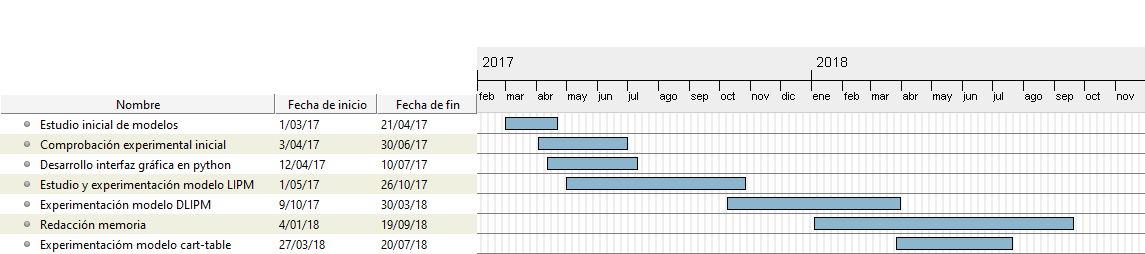
\includegraphics[scale=0.5]{imagenes/apartado_1/12_planificacion_v1}
\caption{Planificación del proyecto}
\label{figura2}
\end{figure}

\begin{enumerate}

\item \textbf{Estudio inicial de modelos trabajados}

En esta fase inicial se realizó un estudio para una toma de contacto con los modelos empleados.

\item \textbf{Comprobación experimental inicial}

A continuación se realizaron una serie de experimentos iniciales para poder comprobar el ajuste de ambos modelos al punto de equilibrio deseado.

\item \textbf{Desarrollo de interfaz gráfica en python}

Se diseñó una interfaz gráfica en python tanto de las fuerzas de los sensores de los tobillos como de las aceleraciones de la imu, detallados en el anexo %%poner el número del anexo en el que inluiré el enlace a dichos archivos .py

\item \textbf{Estudio y experimentación modelo LIPM}

Una vez que se escogió el modelo LIPM como modelo a mejorar, se realizó un estudio y una batería de experimentos para ajustar su respuesta.

\item \textbf{Experimentación modelo DLIPM}

Una vez desarrollado el nuevo modelo Dynamic LIPM, se llevaron a cabo una serie de experimentos para comprobar su validez.

\item \textbf{Estudio y experimentación modelo cart-table}

Por último, se estudió y experimentó con el modelo car-table para mejorar su respuesta ante pequeñas perturbaciones.

\end{enumerate}

\afterpage{\null\newpage}
\newpage


\section{Estado del arte}

\subsection{Origen de la robótica}
La palabra ``Robótica'' fue acuñada por Isaac Asimov para describir la ciencia que se encarga de estudiar la tecnología de los robots. Procede de las palabras checas robota (trabajo forzado) y robotnik
(sirviente) \cite{ref2}.

El término ``robot'', que procede de la palabra robota, se popularizó gracias a la obra literaria Rossum’s Universal Robot (R.U.R.), escrita por Karel Čapek en 1920 \cite{ref3}.

Según la definición de la Organización Internacional de Estándares (ISO) se considera un robot como un: 

``Mecanismo accionado programable en dos o más ejes con un gradio de autonomía, moviéndose dentro de su entorno, para realizar las tareas previstas'' \cite{ref4}. 

A la hora de hablar del concepto de robótica en general, hay que distinguir entre robótica INDUSTRIAL y robótica de SERVICIO. Esta distinción es fundamental a la hora de su desarrollo, fabricación y comercialización.

Según la norma ISO 8373, la definición de robótica INDUSTRIAL es la siguiente:

``Manipulador multifuncional, controlado automáticamente, reprogramable en tres o más ejes, que puede estar fijo o móvil para uso en aplicaciones de automatización industrial''.

En cuanto a lo que respecta a la robótica de SERVICIO, el Comité ISO TC 184/SC2 lo define como:

``Todo tipo de robot que no es industrial''.

A su vez, la IFR proporciona la siguiente definición:

``Robot que opera de forma parcial o totalmente autónoma al servicio del bienestar de los seres humanos y de equipamientos, excluyendo operaciones manufactureras'' \cite{ref5}.

\newpage

\subsubsection{Tipos de robots}

Resulta complicado establecer una clasificación exacta de los robots debido a la gran cantidad de ellos que existe, por lo que se pueden clasificar de forma más general según su arquitectura \cite{ref6}. 

\begin{enumerate}

\item \textbf{Poliarticulados}\\ A este grupo pertenecen los robots cuya característica común es el sedentarismo, aunque pueden ser guiados de forma limitada para poder desplazarse, y cuya estructura se basa en el movimiento de sus elementos terminales para operar en entornos de trabajo fijos, con uno o más sistemas de coordenadas y con un número determinado de grados de libertad. En este grupo se encuentran principalmente los llamados Robots Industriales,como se muestra en la figura \eqref{figura1}, diseñados para operar en entornos repetitivos y sin interacción humano-robot. También pertenecen los manipuladores y los Robots cartesianos, empleados para abarcar amplias zonas de trabajo, actuar sobre diferentes objetos o reducir el espacio ocupado en el suelo.

\begin{figure}[H]
\centering
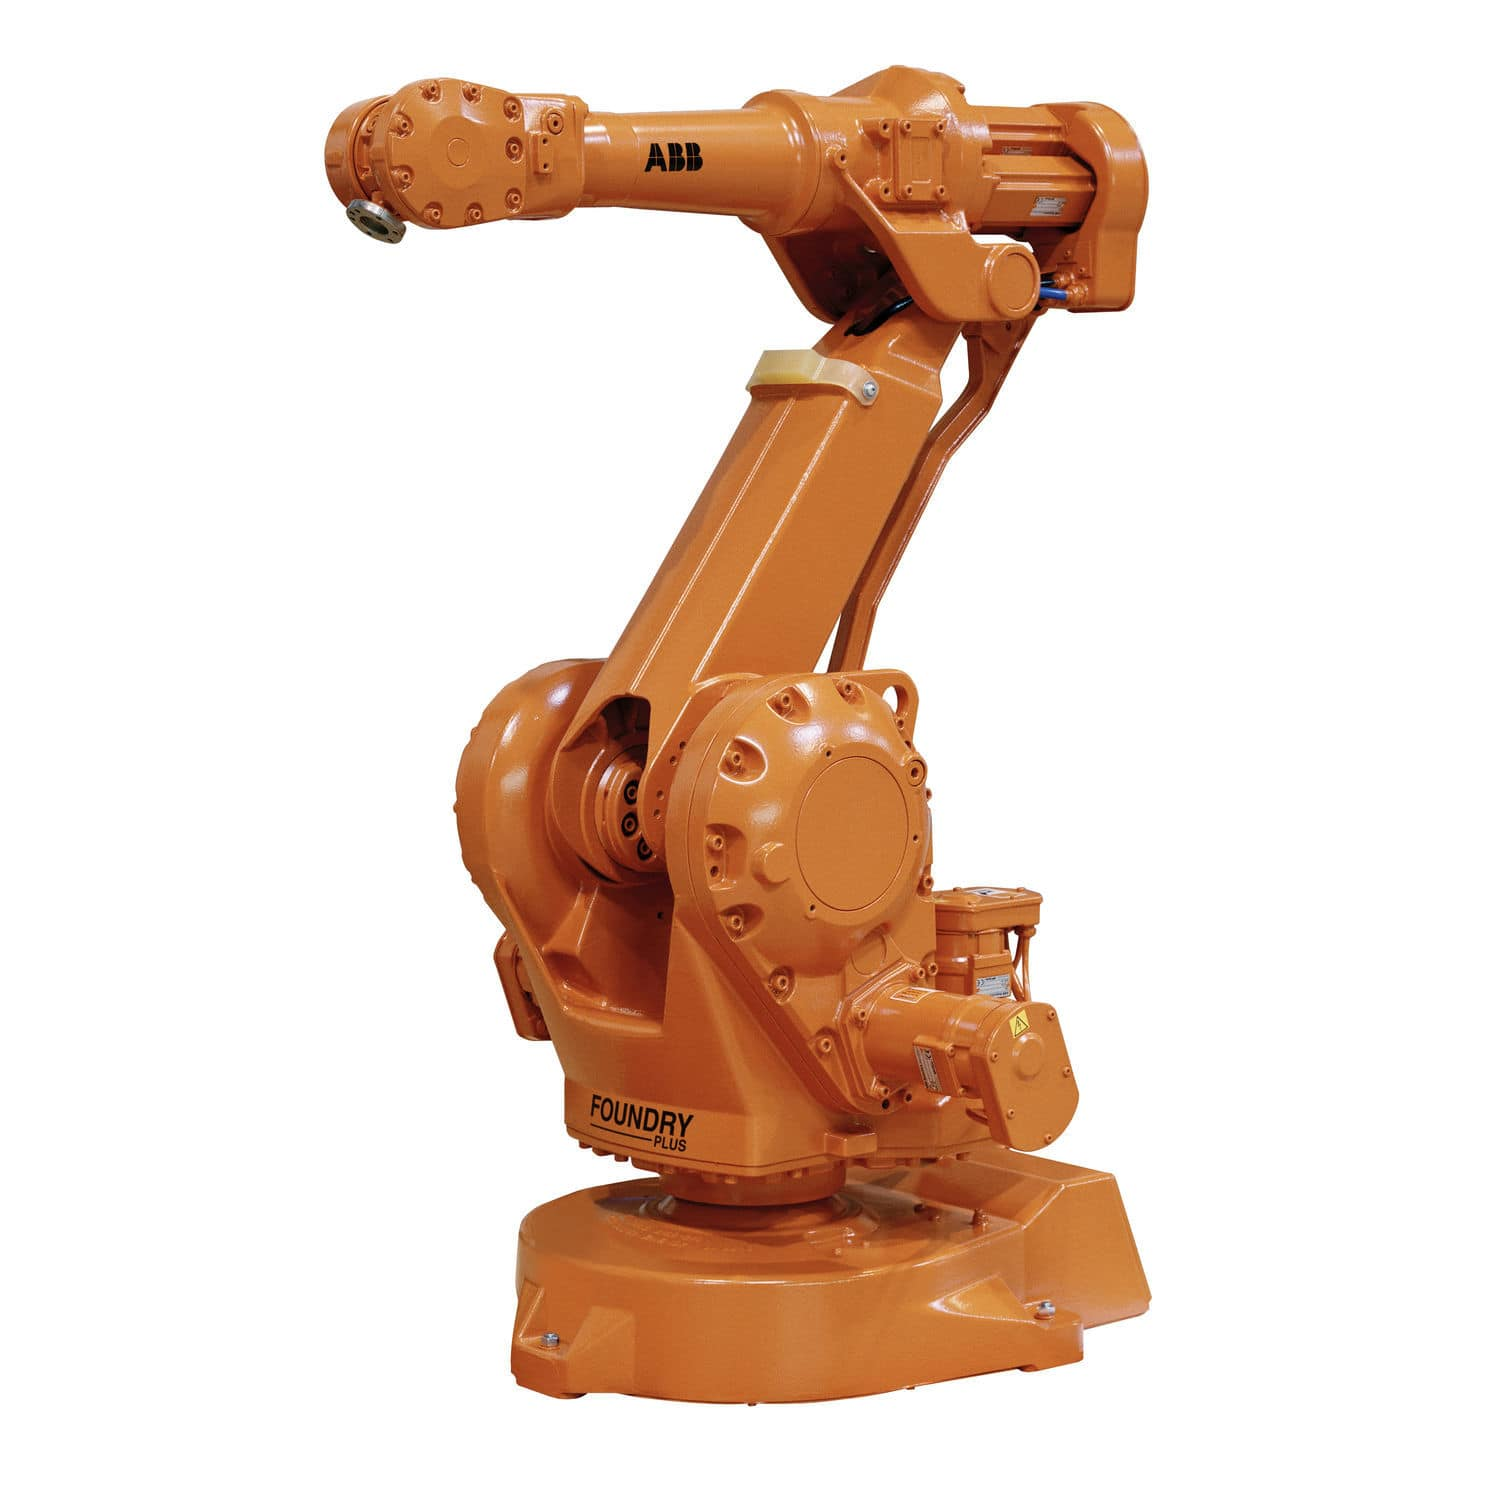
\includegraphics[scale=0.12]{imagenes/apartado_2/21_poliarticulado1_Robot_Industrial_ABB}
\caption{Robot Industrial ABB}
\label{figura21}
\end{figure}

\item \textbf{Móviles}\\ Son robots con capacidad de desplazarse, ya sea mediante ruedas o cualquier plataforma que permita dicha característica, gracias a un sistema motor de tipo rodante. Pueden ser guiados o autónomos (se guían por la información recibida del exterior mediante un sistema de sensores integrado). Estos robots se encargan normalmente de transportar piezas de un punto a otro de la cadena de producción, guiados mediante pistas materializadas a través de la radiación electromagnética de circuitos empotrados en el suelo, o a través de bandas detectadas fotoeléctricamente, otros pueden sortear obstáculos y están dotados de un nivel relativamente elevado de inteligencia.

\begin{figure}[H]
\centering
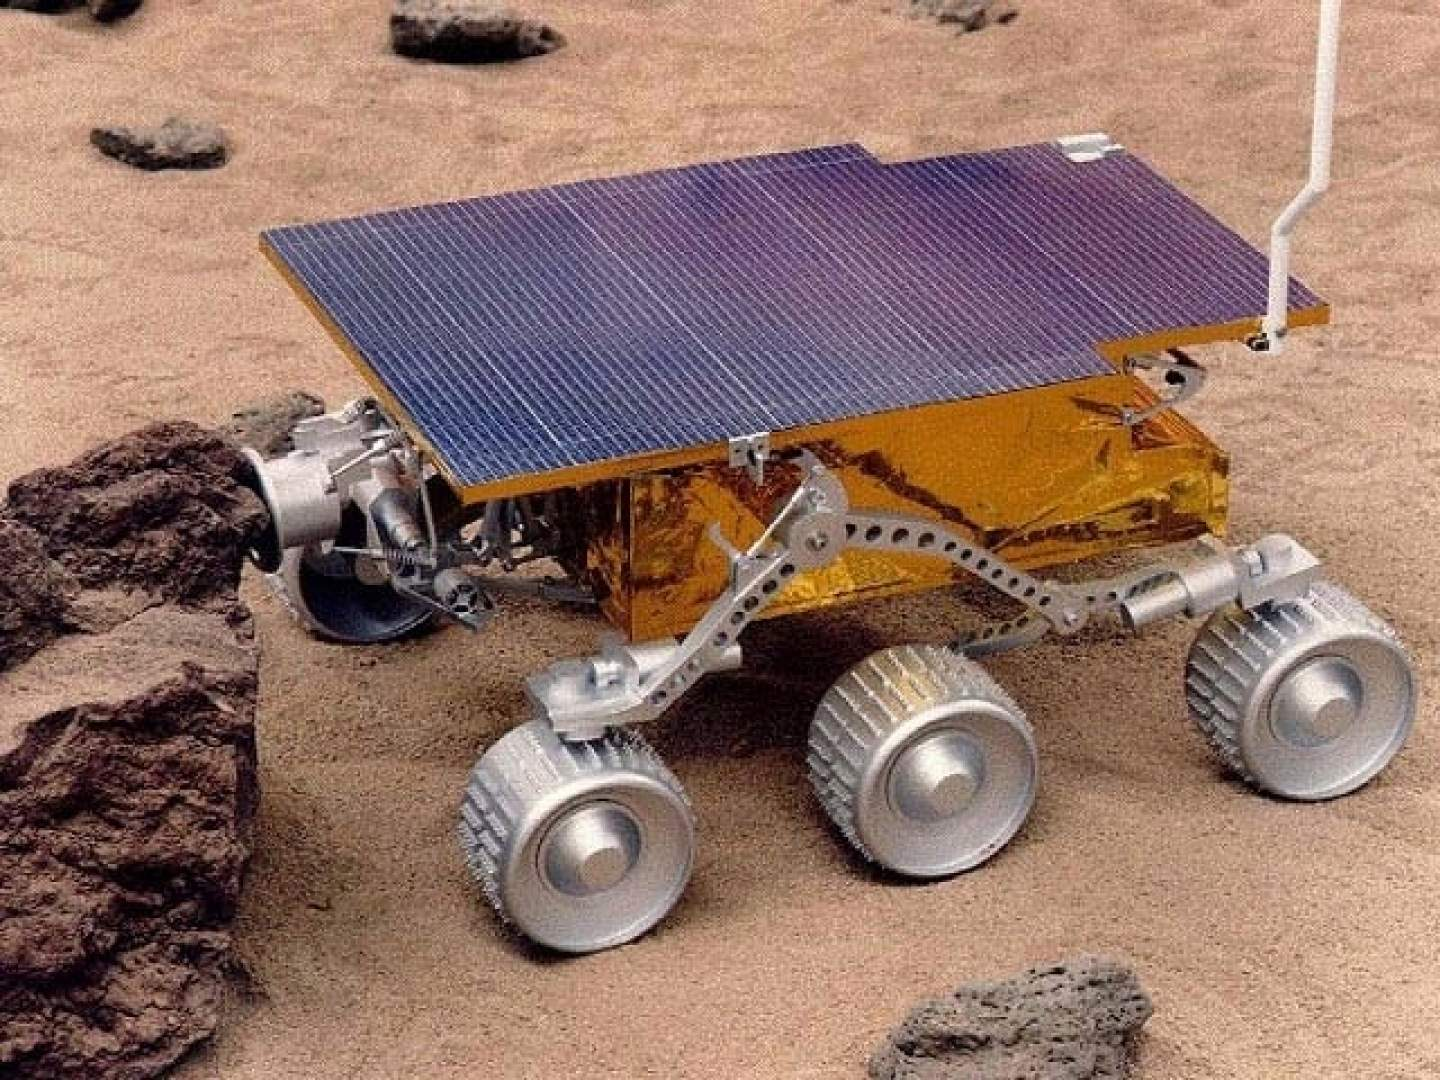
\includegraphics[scale=0.15]{imagenes/apartado_2/22_movil2}
\caption{Mars Pathfinder Rover Sojourner}
\label{figura22}
\end{figure}

\item \textbf{Antropomórficos}\\ Son robots que tratan de imitar parcial o totalmente las acciones y el comportamiento de los seres humanos. Una de las acciones más complejas de éstos es la locomoción bípeda, sobre la que se centra este proyecto y la mayoría de los trabajos en la actualidad, por lo que se concentran en áreas como la investigación y el estudio. El problema que surge es el control dinámico en tiempo real y el mantenimiento simultáneo del equilibrio del robot en dicho proceso.

\begin{figure}[H]
\centering
\subfigure[Robot ASIMO]
{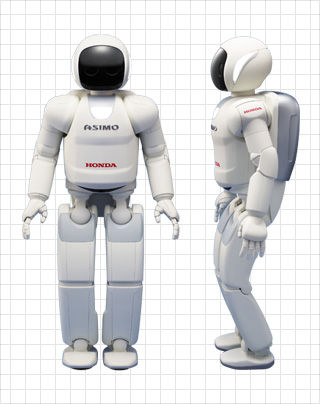
\includegraphics[scale=0.4]{imagenes/apartado_2/23_1_androide1_asimo}}
\quad
\subfigure[Robot TEO]
{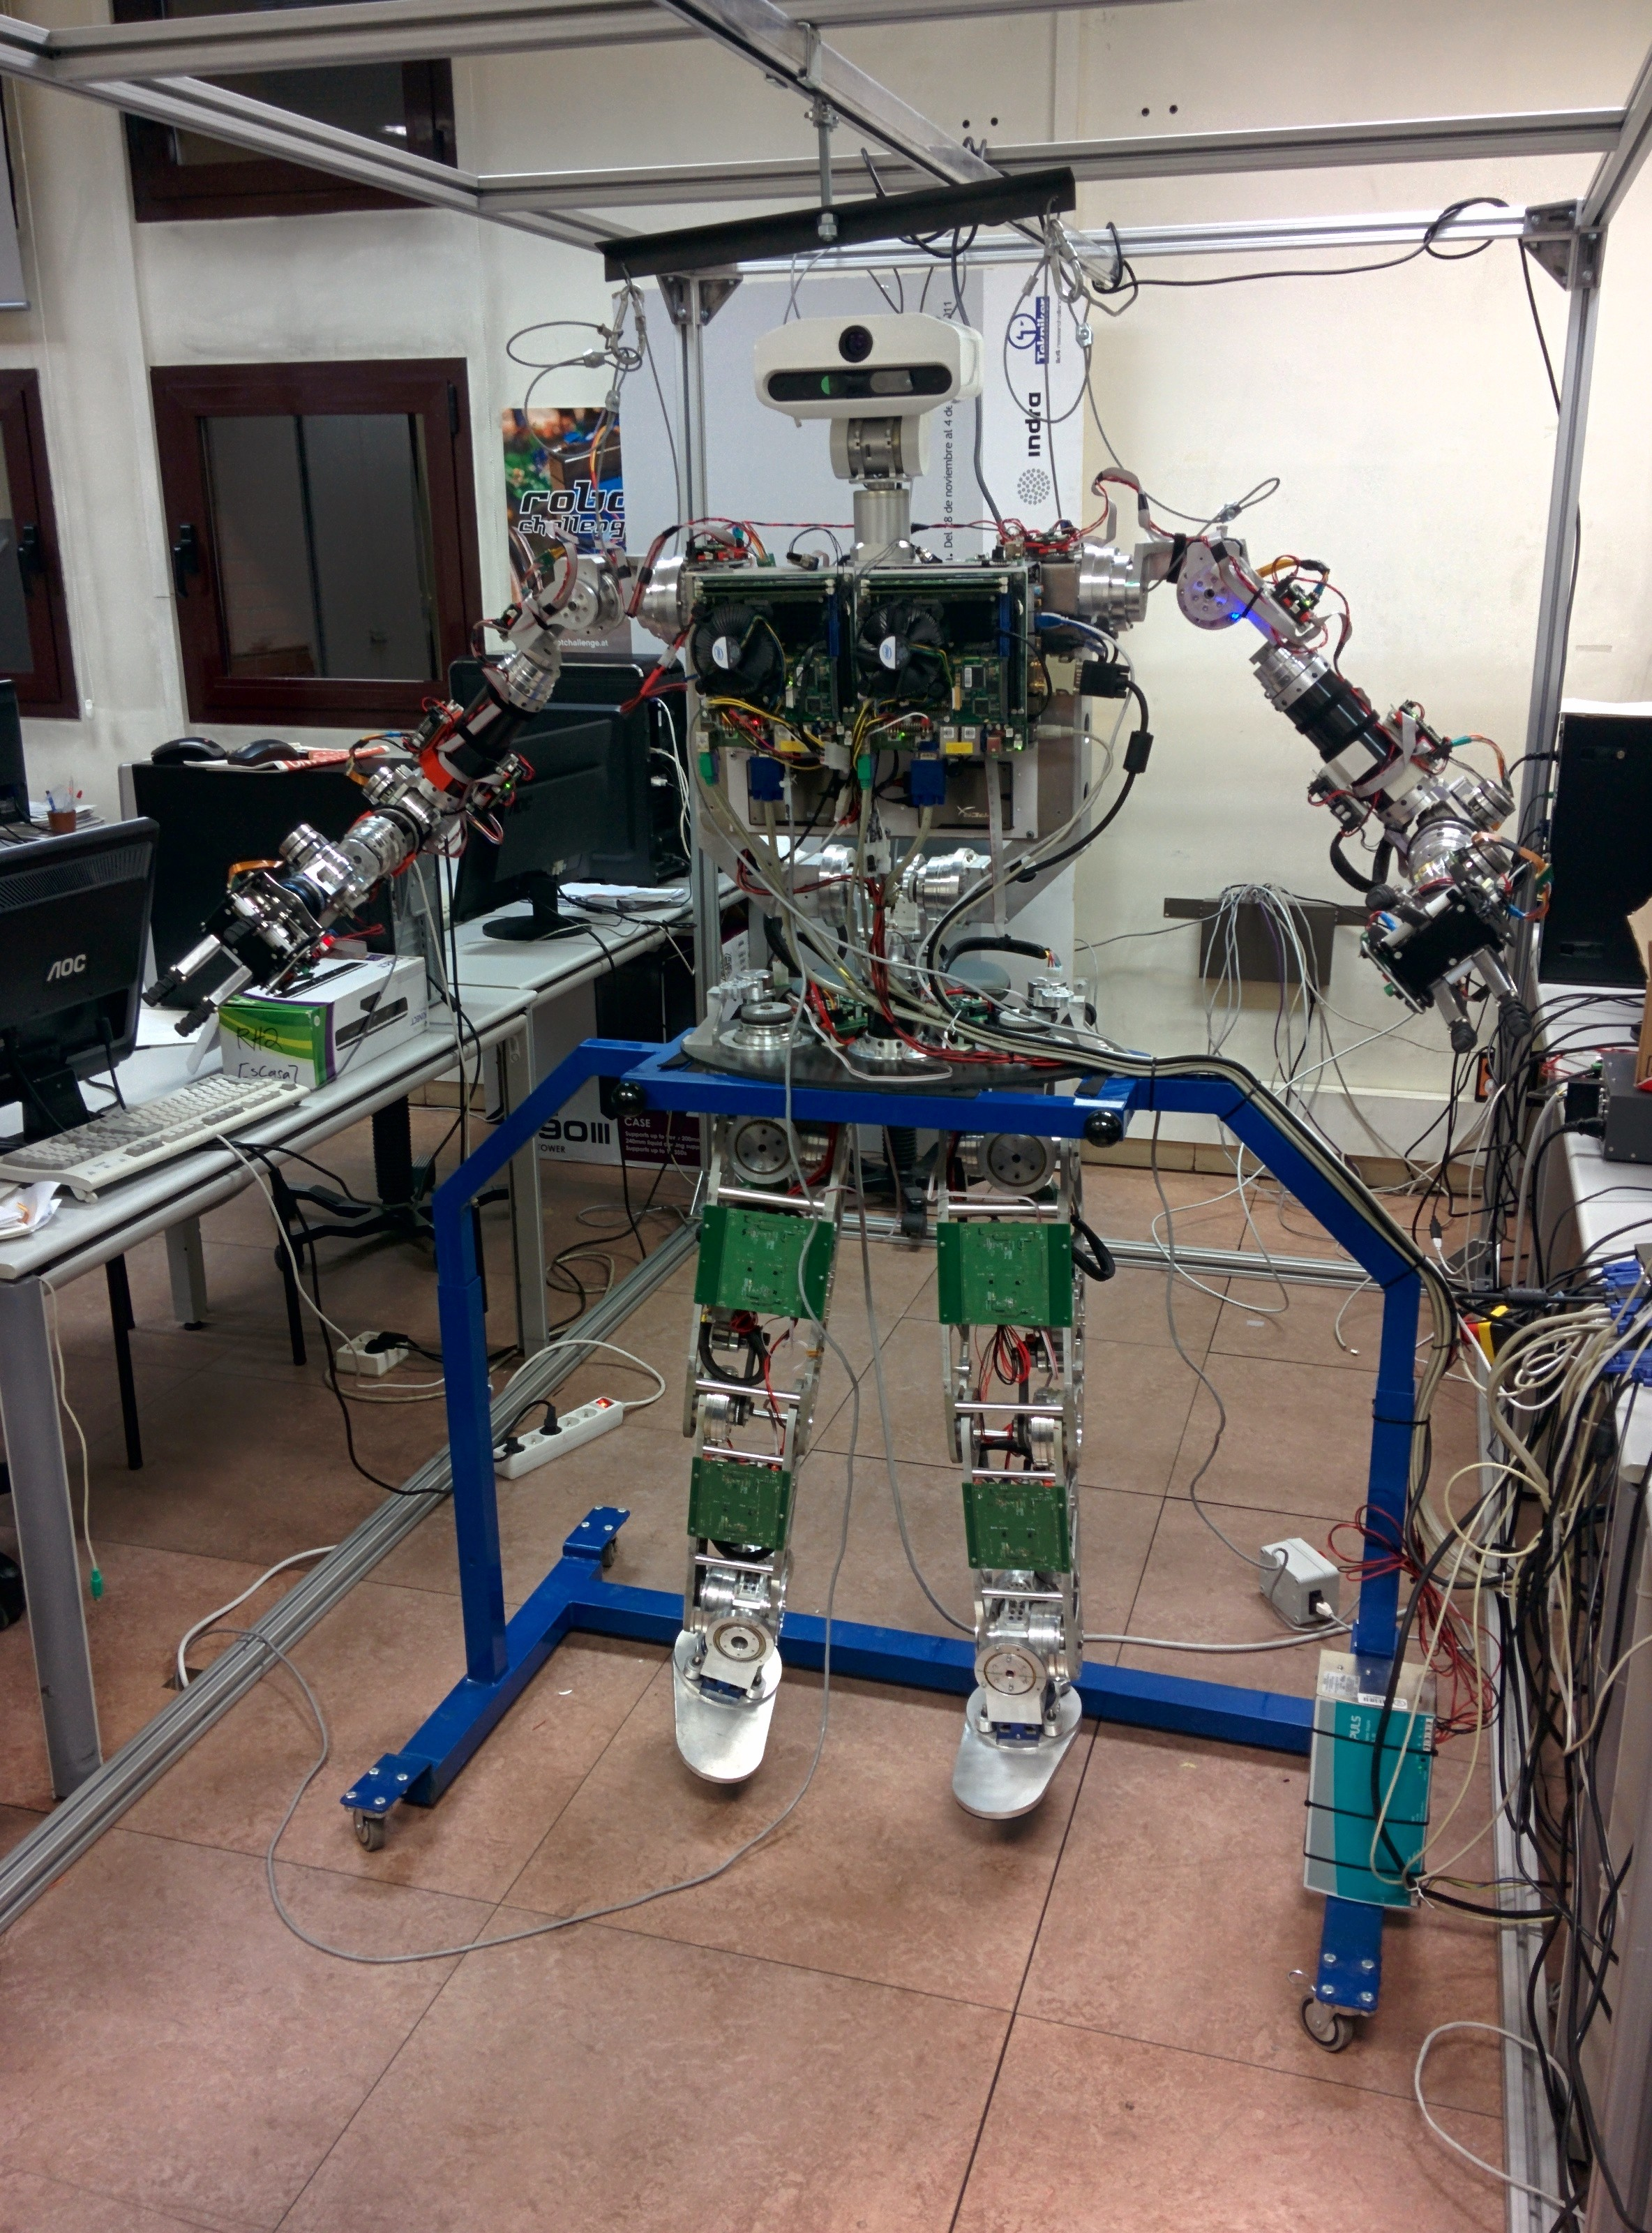
\includegraphics[scale=0.05]{imagenes/apartado_2/23_2_androide2_teo1}}
\caption{Robots antropomórficos}
\label{figura23}
\end{figure}

\item \textbf{Zoomórficos}\\ Son aquellos cuyos sistemas de locomoción imitan a los animales principalmente. Este grupo se podría clasificar en: caminadores y no caminadores.

El grupo de los caminadores es el que más desarrollado está, ya que pueden tener aplicaciones en muchos campos como puede ser el desarrollo de vehículos todoterreno, controlados o autónomos, capaces de avanzar por terrenos con mucho desnivel y accidentados.

Por el contrario, el grupo de los no caminadores es muy escaso y está poco evolucionado. Se han realizado diversos experimentos en Japón con robots de este tipo constituidos por segmentos cilíndricos biselados acoplados axialmente entre sí, capaces de realizar movimientos relativos de rotación.

\begin{figure}[H]
\centering
\subfigure[Robot caminador ANYmal]
{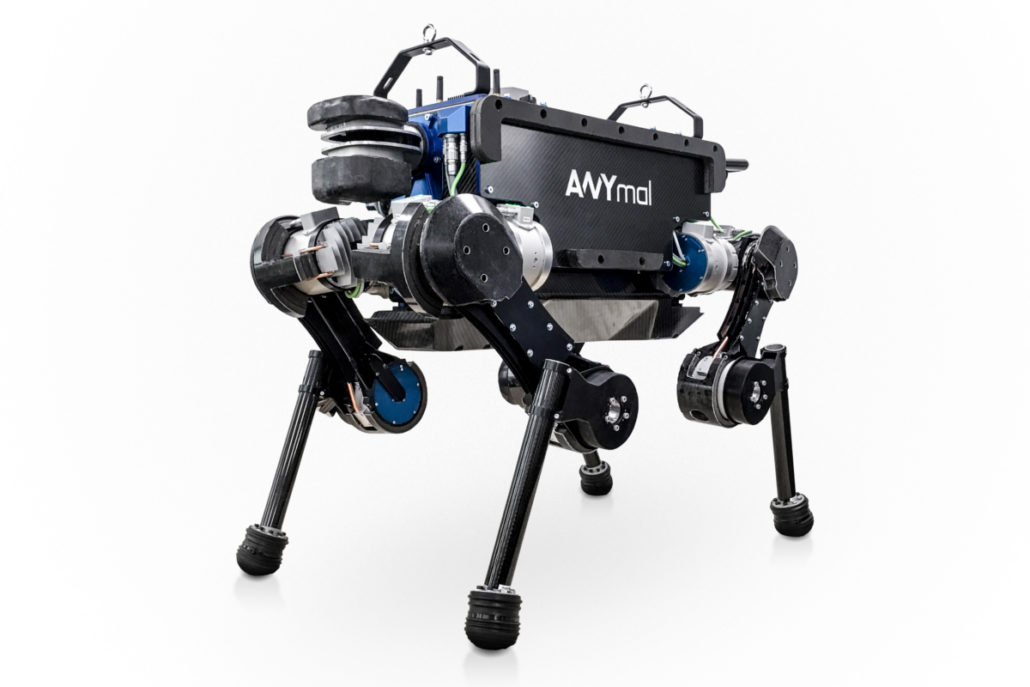
\includegraphics[scale=0.2]{imagenes/apartado_2/24_1_zoomorfico1_ANYmal}}
\quad
\subfigure[Serpiente Robot Modular no caminador]
{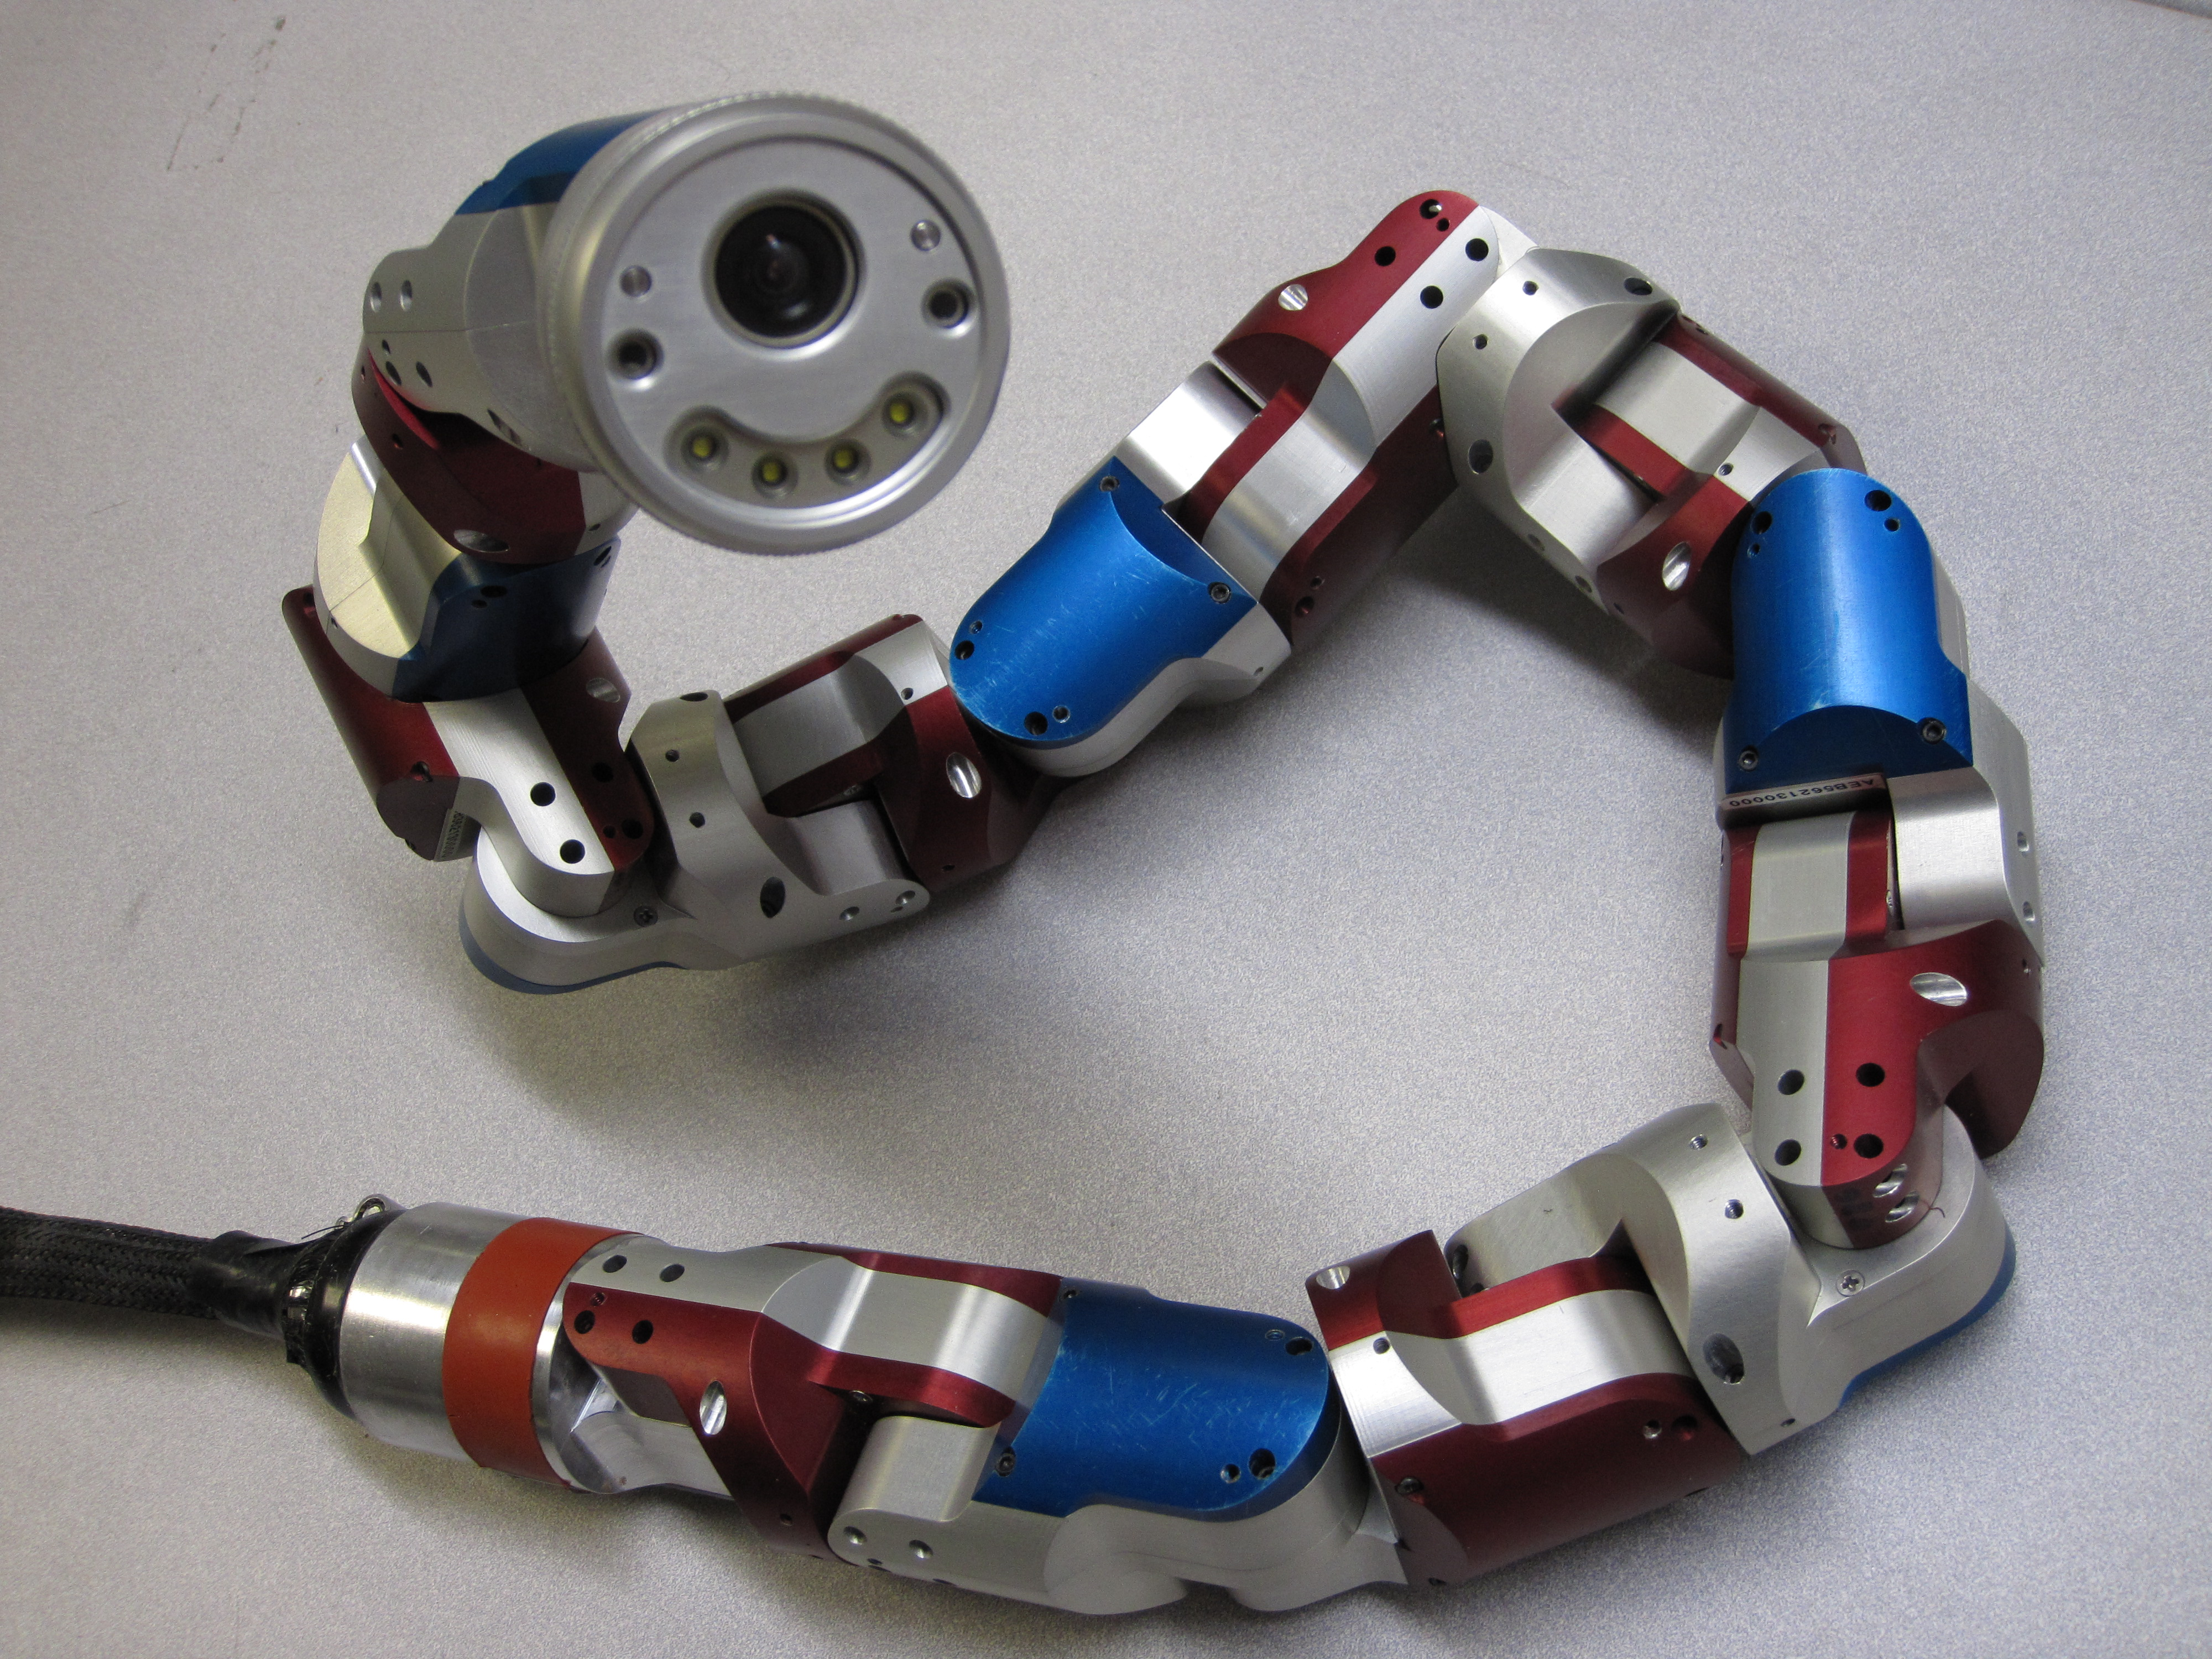
\includegraphics[scale=0.1]{imagenes/apartado_2/24_2_zoomorfico2}}
\caption{Robots zoomórficos}
\label{figura24}
\end{figure} 

\item \textbf{Híbridos}\\ A este grupo pertenecen aquellos Robots que posean en su estructura una combinación de las anteriores ya expuestas, bien sea por conjunción o por yuxtaposición. 

Por ejemplo, un dispositivo con ruedas y con brazos, siendo características de los Robots móviles y de los androides al mismo tiempo \footnote{Imágenes sacadas de \cite{ref36}, \cite{ref37} y wikipedia}.

\begin{figure}[H]
\centering
{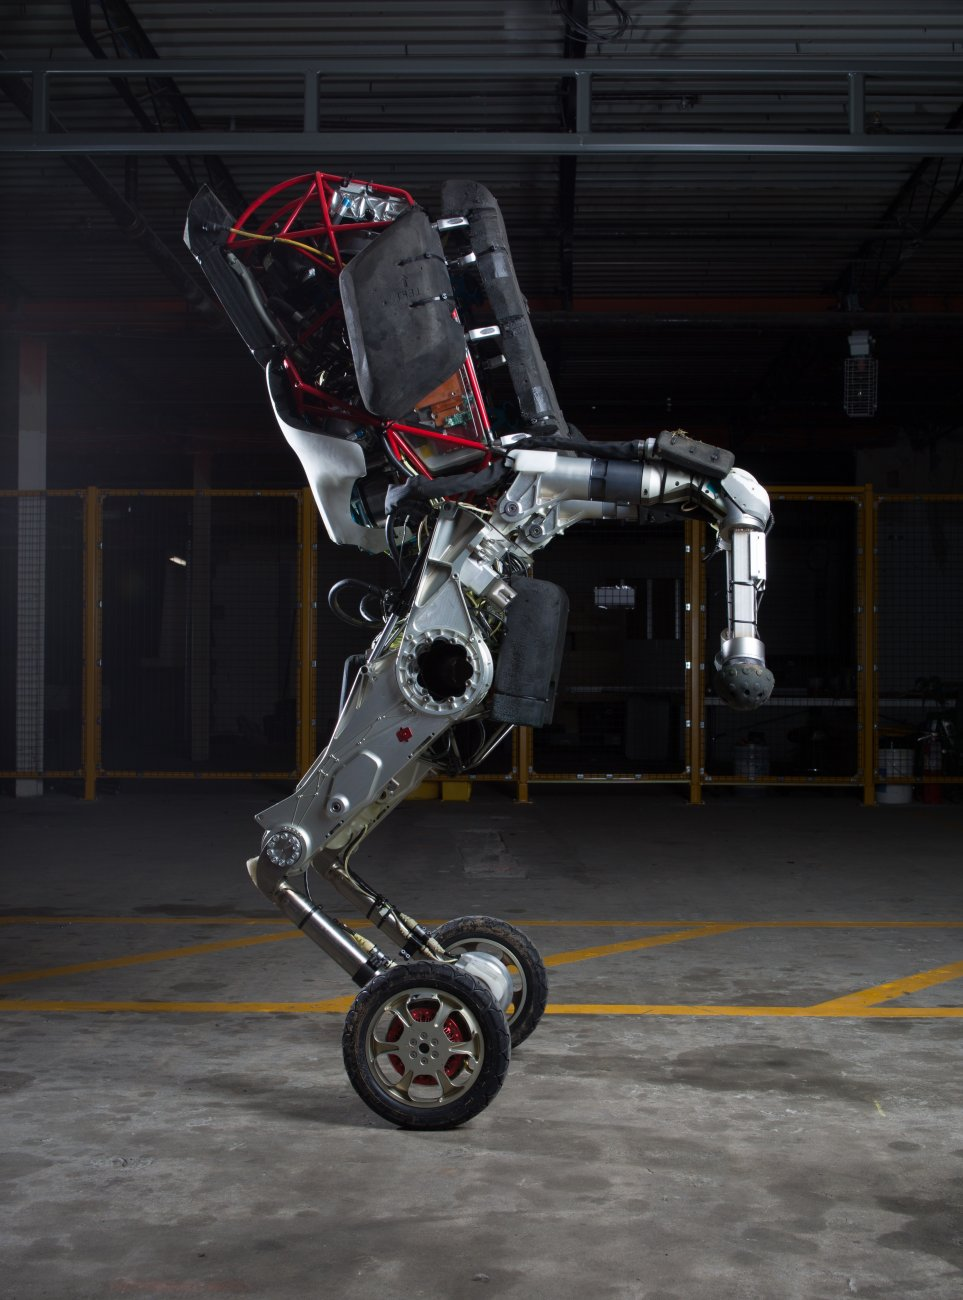
\includegraphics[scale=0.15]{imagenes/apartado_2/25_hibrido_handle_bd}}
\caption{Robot HANDLE}
\label{figura25}
\end{figure}

\end{enumerate}

\newpage

\subsection{Evolución de los Robots Humanoides}\label{historia_robots_humanoides}

El desarrollo de los robots humanoides ha sido largo y complejo.

Hubo que esperar al año 1495 para tener los primeros registros del que posiblemente sea el primer robot humanoide, diseñado y construido por Leonardo da Vinci. Se trataba de un robot mecánico, un guerrero vestido con una armadura, que podía realizar movimientos similares a los de los seres humanos como sentarse, mover los brazos y girar la cabeza y el cuello \cite{ref7}.

\begin{figure}[H]
\centering
{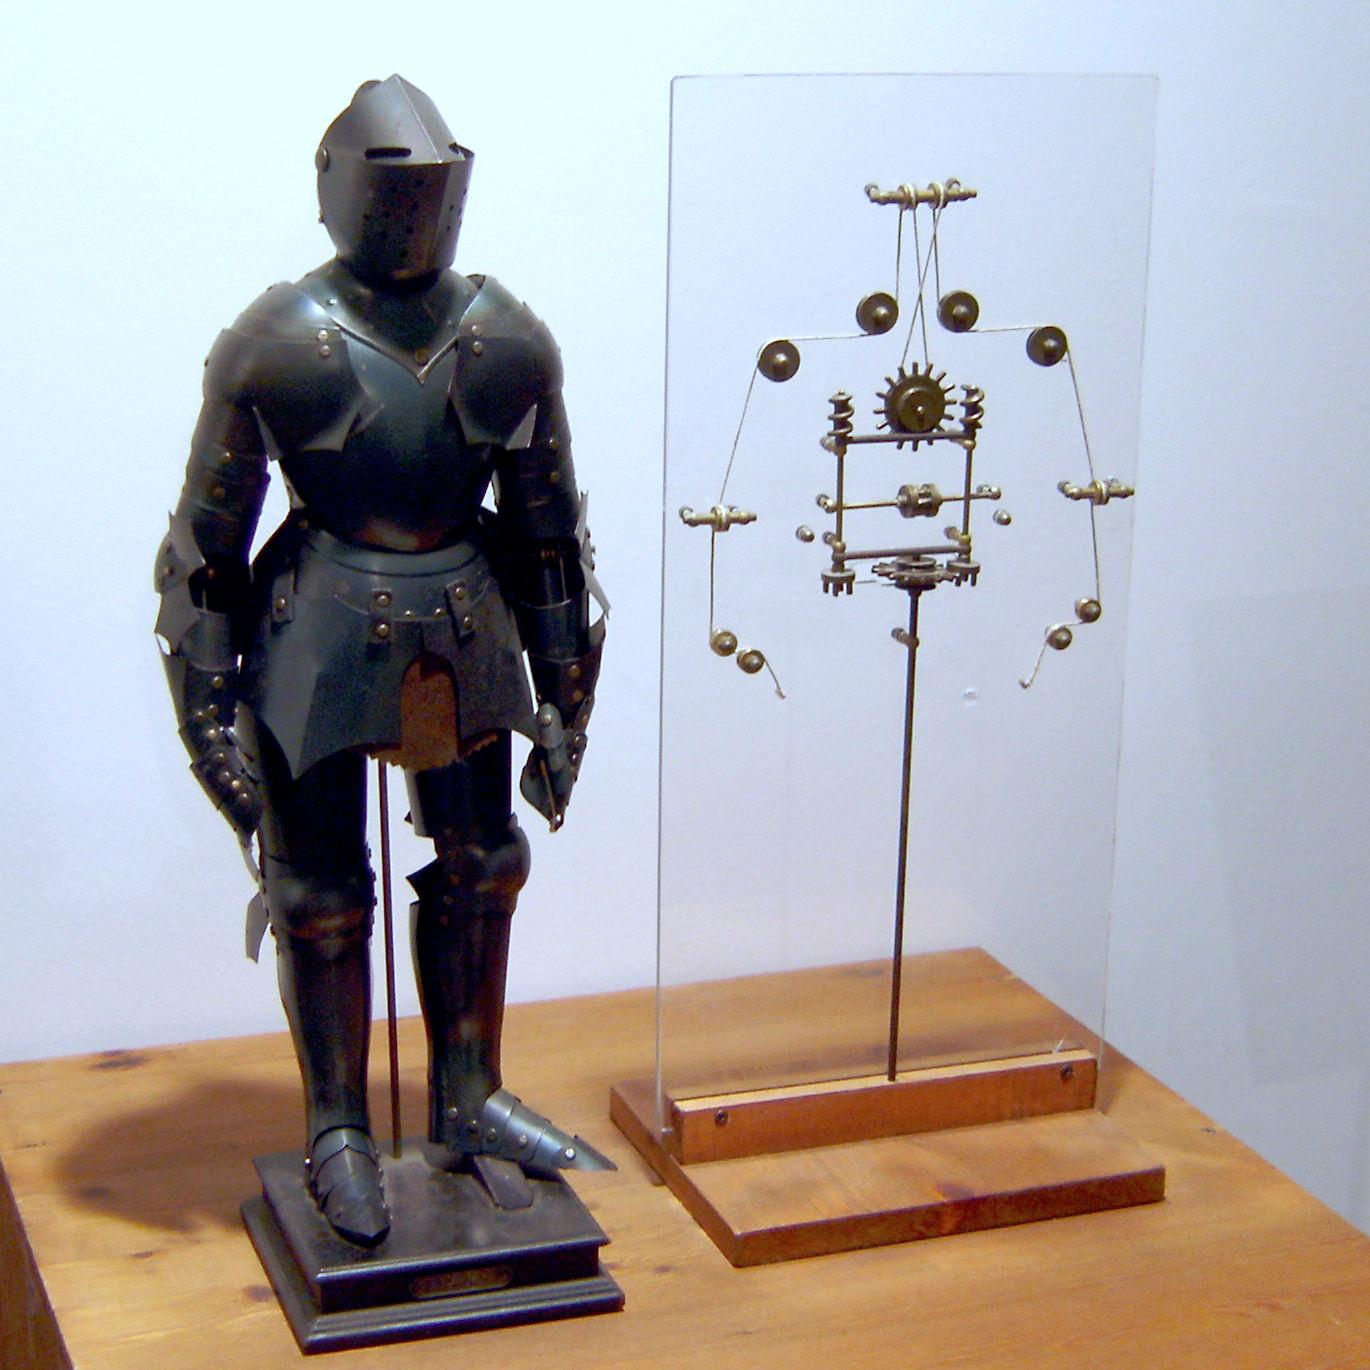
\includegraphics[scale=0.1]{imagenes/apartado_2/26_robot_LeonardoDaVinci}}
\caption{Armadura diseñada por Leonardo Da Vinci}
\label{figura26}
\end{figure}

El siglo XVIII fue una época prolífica para el desarrollo de robots autónomos. En 1773, Pierre y Henry Louis inventaron la primera máquina autónoma capaz de escribir.

Pero cuando empieza realmente el desarrollo de los robots humanoides fue a partir del siglo XIX. Uno de los primeros fue el trompetista mecánico, construido por Fridrich Kaufmann en 1810, que contenía un tambor con muescas que usaba para activar algunas válvulas que ayudaban a pasar el aire a través de doce lenguas, lo que producía un tipo de sonido modulado que a su vez pasaba por una trompeta, para hacerla sonar. En 1865 John Brainerd inventó el hombre de vapor, movido por una máquina de vapor que tiraba de unos carros. En 1855 Frank Reade Junior construyó al llamado Hombre Eléctrico, una versión electrificada del hombre de vapor.

\begin{figure}[H]
\centering
{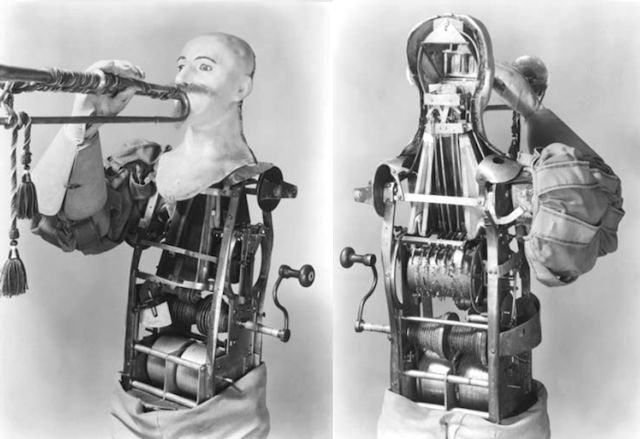
\includegraphics[scale=0.3]{imagenes/apartado_2/27_trompetista_mecanico}}
\caption{Trompetista mecánico}
\label{figura27}
\end{figure}

A partir del siglo XX el número de robots humanoides fue aumentando y evolucionando. Uno de los primeros fue ELEKTRO, desarrollado por la sociedad Westinghouse en 1938, un robot más cerca del concepto de humanoide que podía caminar controlado por comandos de voz, y hablaba gracias a un tocadiscos de 78 rpm. Más tarde se le unió ``Sparko'', un perro robot capaz de sentarse, ladrar y suplicar. 

\begin{figure}[H]
\centering
{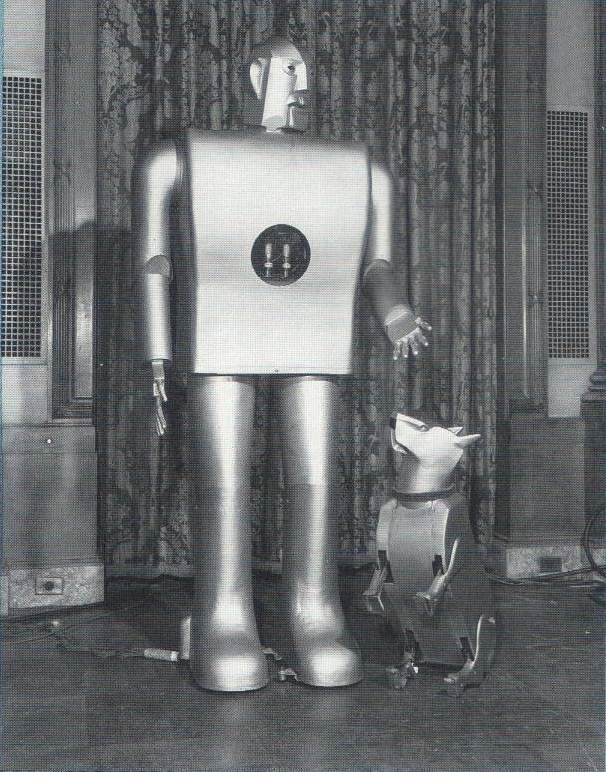
\includegraphics[scale=0.2]{imagenes/apartado_2/28_elektro_robot}}
\caption{Robot Elektro}
\label{figura28}
\end{figure}

Durante las décadas de los 60's a los 90's aparecieron numerosos robots bípedos. El profesor Kato del equipo robótico de la Universidad de Waseda en Japón desarrolló varias familias de robots bípedos. La primera fue llamada Waseda Legged (WL), que se caracterizaba por ser robots compuestos de sólo dos piernas. En 1969, con la aparición del músculo artificial de goma, desarrollaron la serie WAP (Waseda's Anthropomorphic Pneumatically-activated pedipulators), activados mediante el control de dichos músculos. No fue hasta el modelo WAP-3 que consiguieron que el robot bípedo se desplazara en 3 dimensiones, ya que los dos primeros modelos sólo se movían en un plano.

\begin{figure}[H]
\centering
\subfigure[WL-1]
{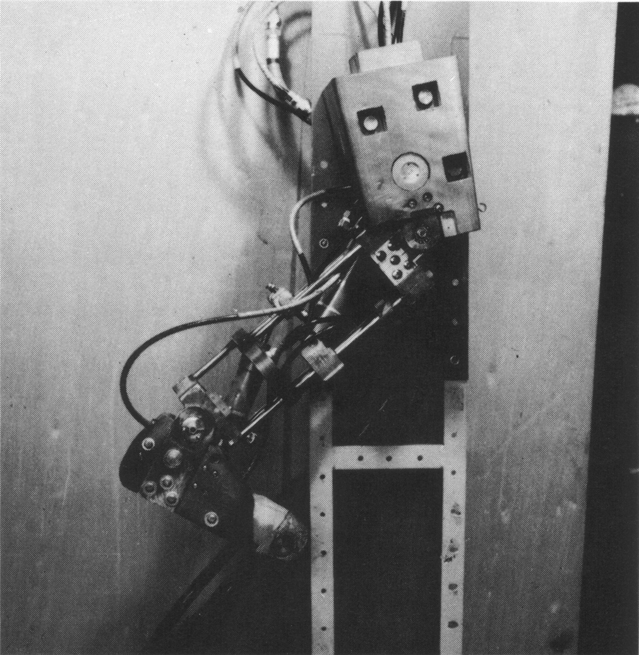
\includegraphics[scale=0.5]{imagenes/apartado_2/29_1_WL_1_1967}}
\quad
\subfigure[WL-3]
{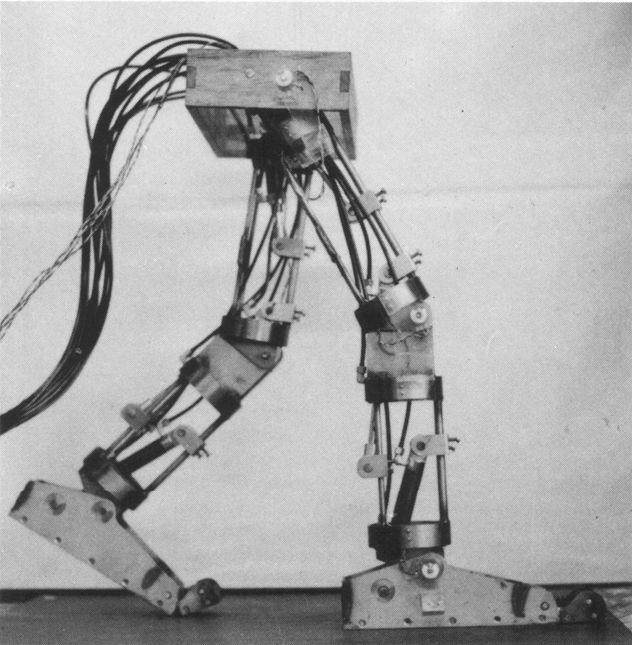
\includegraphics[scale=0.5]{imagenes/apartado_2/29_2_WL_3_1969}}
\caption{Robots Waseda Legged}
\label{figura29}
\end{figure}

\begin{figure}[H]
\centering
\subfigure[WAP-1]
{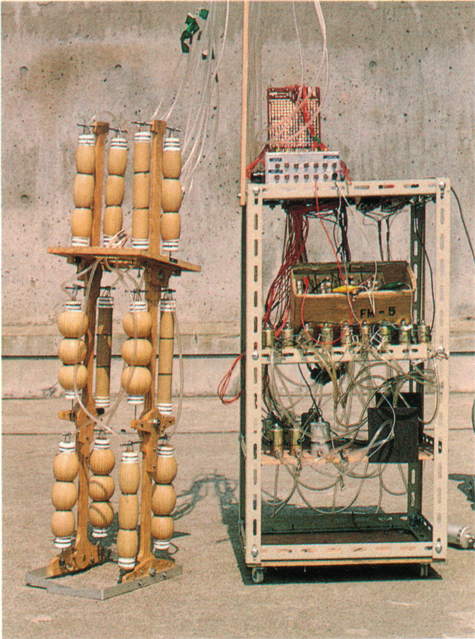
\includegraphics[scale=0.6]{imagenes/apartado_2/210_1_WAP_1_1969}}
\quad
\subfigure[WAP-2]
{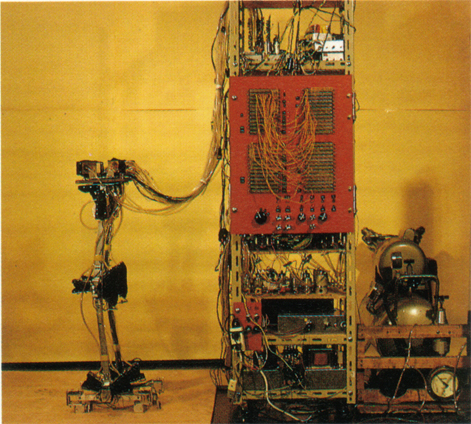
\includegraphics[scale=0.8]{imagenes/apartado_2/210_2_WAP_2_1970}}
\quad
\subfigure[WAP-3]
{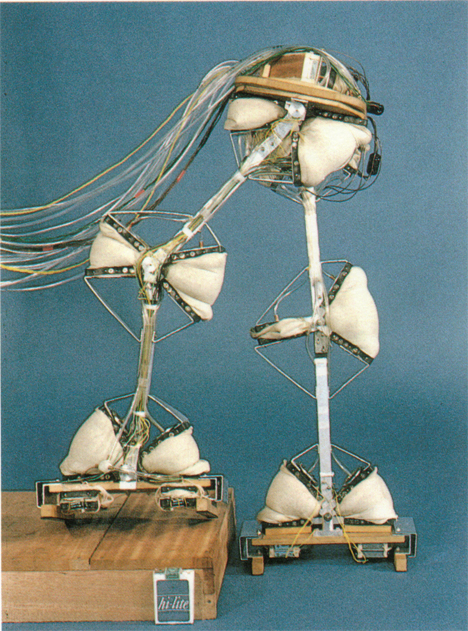
\includegraphics[scale=0.6]{imagenes/apartado_2/210_3_WAP_3_1971}}
\caption{Waseda's Anthropomorphic Pneumatically-activated pedipulators}
\label{figura210}
\end{figure}

Ya en 1970, con los avances en la investigación de robots antropomórficos inteligentes, aparecieron los primeros robots con torso y piernas, pareciéndose cada vez más a los seres humanos. De estos avances se desarrollaron los robots de la familia WABOT (WAseda roBOT), basados en sistemas de control de extremidades, visión y sistemas de conversación. El WABOT-2 incluso era capaz de leer partituras y tocar un teclado.

\begin{figure}[H]
\centering
\subfigure[WABOT-1]
{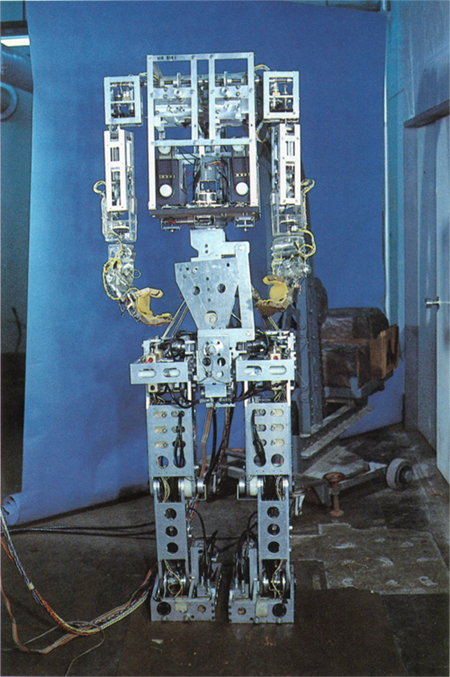
\includegraphics[scale=0.6]{imagenes/apartado_2/211_1_WABOT_1_1973}}
\quad
\subfigure[WABOT-2]
{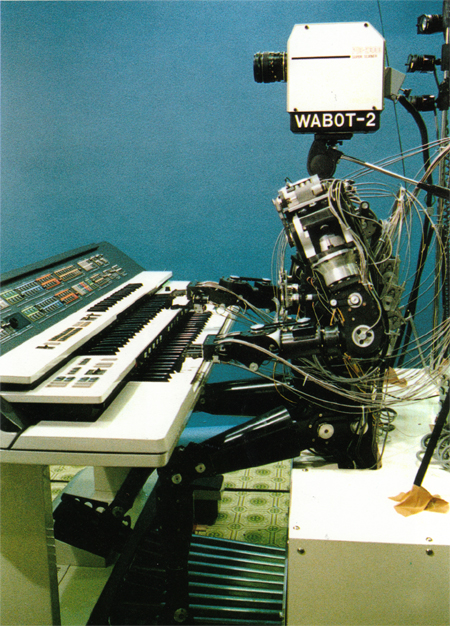
\includegraphics[scale=0.65]{imagenes/apartado_2/211_2_WABOT_2_1984}}
\caption{Robots antropomórficos inteligentes WAseda roBOT}
\label{figura211}
\end{figure}

Unos años más tarde, en 1996 se desarrolló la familia de robots WABIAN, que se caracterizaban por utilizar motores eléctricos, logrando la misma velocidad de paso que un humano \cite{ref8}.

En Japón la compañía HONDA llevaba desarrollando robots bípedos desde 1986. Primero fueron del modelo E0 al E6, para pasar a los P1 a P3 y terminando por el robot humanoide más inteligente llamado ASIMO, que fue desarrollado en el 2000.

\begin{figure}[H]
\centering
{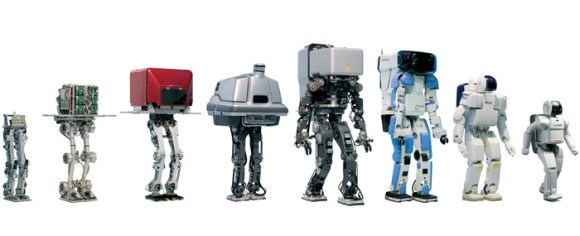
\includegraphics[scale=0.7]{imagenes/apartado_2/212_evolucion_Honda_robots}}
\caption{De izquierda a derecha, E0 hasta ASIMO}
\label{figura212}
\end{figure}

Dos años más tarde, bajo el Ministerio de Económicas, Comercio e Industria de Japón, se desarrolló el Proyecto Humanoide Robot (HRP), con el HRP-2 a la cabeza de la tecnología en esos años \cite{ref22}.

\begin{figure}[H]
\centering
{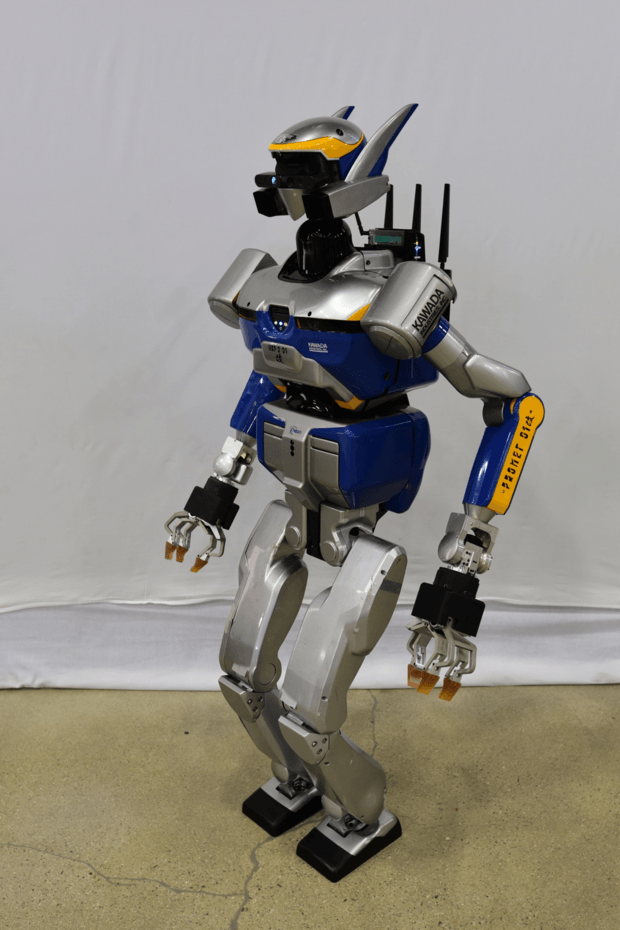
\includegraphics[scale=0.2]{imagenes/apartado_2/213_HRP_2}}
\caption{HRP-2}
\label{figura213}
\end{figure}

En la actualidad, los robots humanoides están muy avanzados, pudiendo incluso correr y mantener el equilibrio. Un ejemplo de ello lo tenemos en ATLAS, desarrollado en 2013 por Boston Dynamics, capaz de caminar por terrenos irregulares sin perder el equilibrio, cargar objetos pesados, e incluso recientemente, dar saltos \cite{ref29}\footnote{Imágenes del apartado \ref{historia_robots_humanoides} están sacadas de \cite{ref34}, \cite{35} y wikipedia}.

\begin{figure}[H]
\centering
{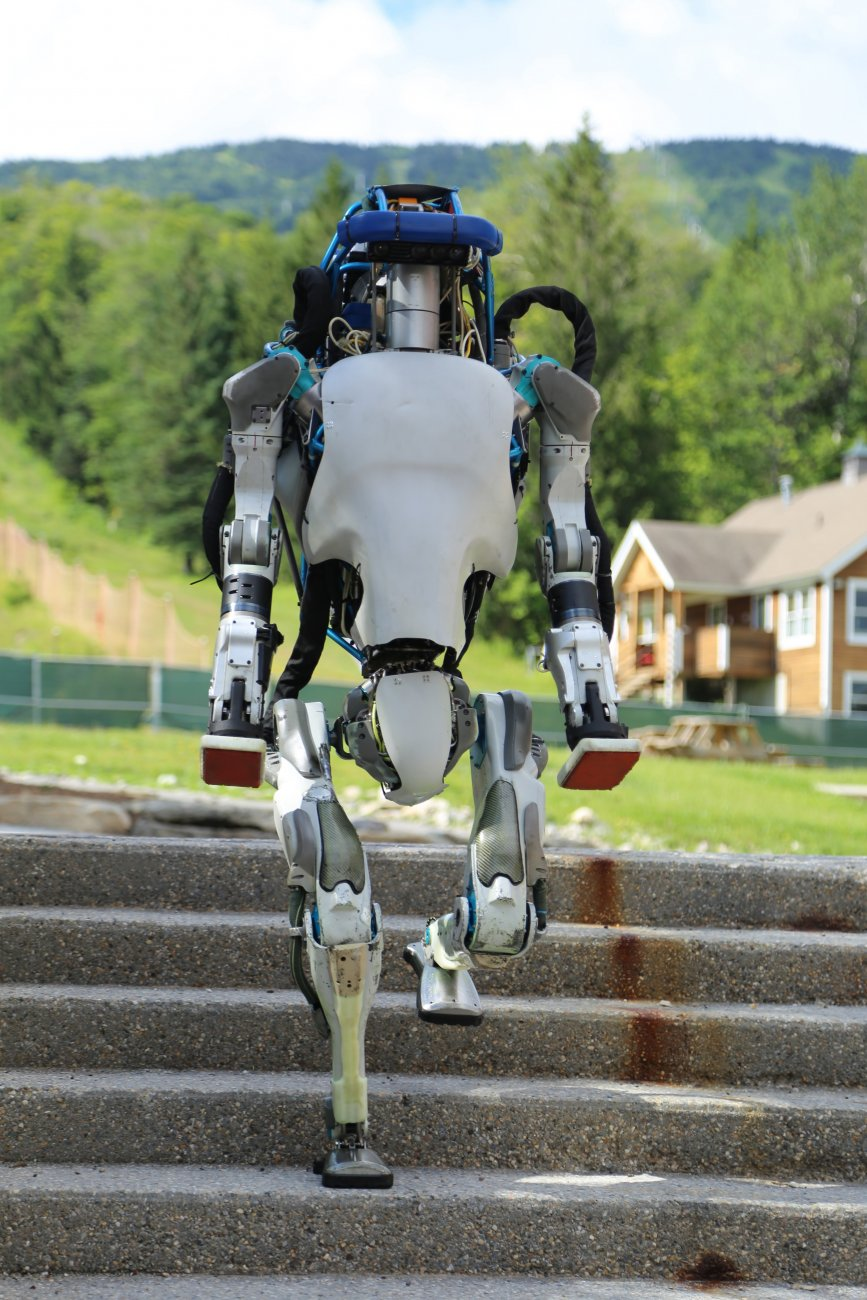
\includegraphics[scale=0.2]{imagenes/apartado_2/214_atlas_boston_dynamics}}
\caption{ATLAS}
\label{figura214}
\end{figure}

\newpage

\subsection{Locomoción bípeda}
%%Definición de centro de masas sacada de http://www2.montes.upm.es/dptos/digfa/cfisica/dinamsist/cdm.html
Para hablar de locomoción bípeda o caminata, primero hay que hacer una introducción de una serie de conceptos para poder entender mejor este movimiento.

\begin{itemize}
\item \emph{Centro de Masas} (CoM): es el punto en el que se concentra toda la masa del sistema y sobre el que actúa la resultante de todas las fuerzas que afectan al sistema \cite{ref9}. Según los modelos CAD del robot TEO, el CoM se encuentra a una altura de 0,893 m.

\begin{figure}[H]
\centering
{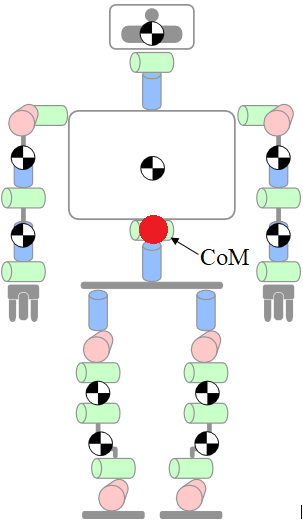
\includegraphics[scale=0.5]{imagenes/apartado_2/215_center_of_mass}}
\caption{Centro de Masas del robot humanoide TEO (en color rojo)}
\label{figura215}
\end{figure}

\item \emph{Polígono de soporte}: se trata del área de contacto de los puntos de apoyo con el suelo. Puede ser simple, con un pie, o doble, con los dos pies.

\begin{figure}[H]
\centering
{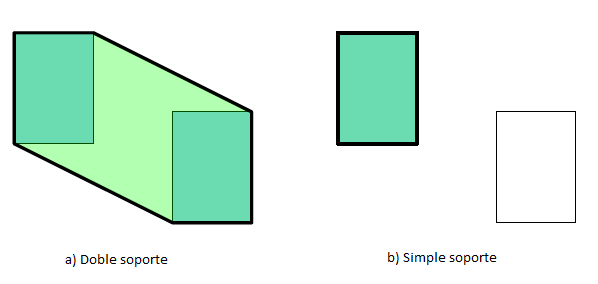
\includegraphics[scale=0.6]{imagenes/apartado_2/216_supportpolygon}}
\caption{Polígono de soporte}
\label{figura216}
\end{figure}

\item \emph{Punto de Momento Cero} (ZMP): Según Vukobratović \cite{ref19}, es el punto $R$ en el cual la suma de momentos es igual a 0.

\begin{figure}[H]
\centering
{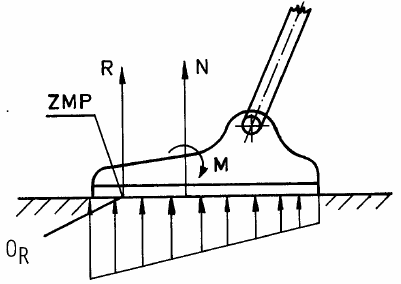
\includegraphics[scale=0.6]{imagenes/apartado_2/217_zmp}}
\caption{ZMP}
\label{figura217}
\end{figure}

\item \emph{Centro de Presión} (CoP): Punto en el polígono de soporte donde actúa la suma total de las fuerzas de contacto, causando una fuerza pero no un momento \cite{ref24}. 

\begin{figure}[H]
\centering
{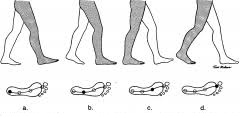
\includegraphics[scale=1.3]{imagenes/apartado_2/218_cop}}
\caption{Evolución del CoP durante el paso}
\label{figura218}
\end{figure}

\item \emph{Pivote del Momento Centroidal} (CMP): Punto donde la fuerza de reacción del suelo actúa manteniendo constante la componente horizontal del momento angular de todo el cuerpo. El CMP es igual al ZMP en el caso en que el momento del CoM es cero. Sin embargo, cuando aparece un momento significativo sobre el CoM, aunque por definición el ZMP no puede abandonar el polígono de soporte en el suelo, el CMP puede hacerlo, como se puede observar en la figura \ref{figura219} \cite{ref25}.

\begin{figure}[H]
\centering
{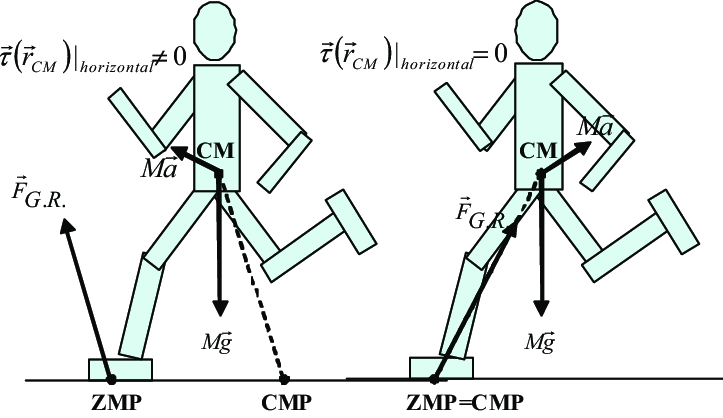
\includegraphics[scale=0.4]{imagenes/apartado_2/219_centroidal_moment_pivot}}
\caption{Pivote del Momento Centroidal (CMP)}
\label{figura219}
\end{figure}

\end{itemize}

\textbf{¿QUÉ ES LOCOMOCIÓN BÍPEDA O CAMINATA?}

La locomoción bípeda, o caminata, es la acción de desplazarse de un lugar a otro manteniendo en todo momento un pie en contacto con la superficie. En lo seres humanos este movimiento complejo y periódico alterna una fase de estabilidad con una fase de inestabilidad. Esta fase de inestabilidad es provocada por la gravedad, pero gracias a ella se produce el movimiento hacia adelante. Debido a la complejidad de este movimiento, se ha utilizado el criterio de Punto de Momento Cero (ZMP) para simplificar su análisis. 

Los robots humanoides han sido desarrollados para imitar los movimientos y comportamientos de los humanos. Pero la caminata resulta un comportamiento muy complejo para éstos. 

Existen dos tipos de caminata, llamadas caminata estática y  caminata dinámica. En la caminata estática el CoM no abandona nunca el polígono de soporte. Sin embargo, en la caminata dinámica, hay periodos en los que la proyección del CoM se sale fuera del polígono de soporte \cite{ref10}, como se puede observar en la figura \ref{figura220}.

\begin{figure}[H]
\centering
{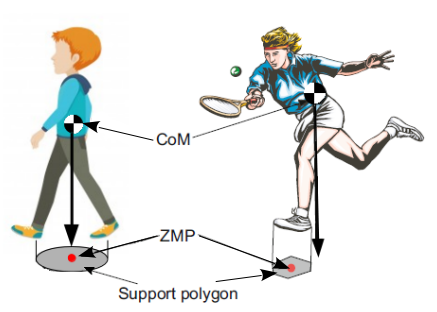
\includegraphics[scale=0.45]{imagenes/apartado_2/220_com_zmp_supportpolygon}}
\caption{CoM, Polígono de soporte y ZMP}
\label{figura220}
\end{figure}

Cuando los seres humanos realizan el movimiento de caminar logran mantener el equilibrio gracias a un control corporal total. Sin embargo los robots humanoides no son capaces de controlar por sí solos su cuerpo, por lo que su control de estabilidad es más complejo. En el actual proyecto se van a explicar dos modelos que desarrollan un controlador para mantener el equilibrio en los robots: el modelo de péndulo invertido y el modelo cart-table. Éstos consisten en calcular ciertos parámetros haciendo uso de los sensores de fuerza-par, en el caso del péndulo invertido, y del sensor inercial, en el caso del cart-table, para lograr mantener el equilibrio en la caminata de los robots.

\textbf{FASES DEL PASO}

En el paso o caminata bípeda, como se puede observar en la figura \ref{figura221}, las fases se distinguen por:

\begin{itemize}
\item \textbf{FASE 1}.Fase de apoyo\\
En esta fase la pierna y el pie que están completamente apoyados en el suelo, soportan todo el peso del bípedo, mientras la pierna de balanceo está realizando el paso.

\item \textbf{FASE 2}.Fase de balanceo\\
En esta fase la pierna y el pie que estaban antes apoyados ahora están realizando un paso (avanzando por el aire), hasta volver al apoyo de nuevo. 

\end{itemize}

%%imagen sacada de https://warwick.ac.uk/fac/sci/eng/meng/nongps/rnd/gait/

\begin{figure}[H]
\centering
{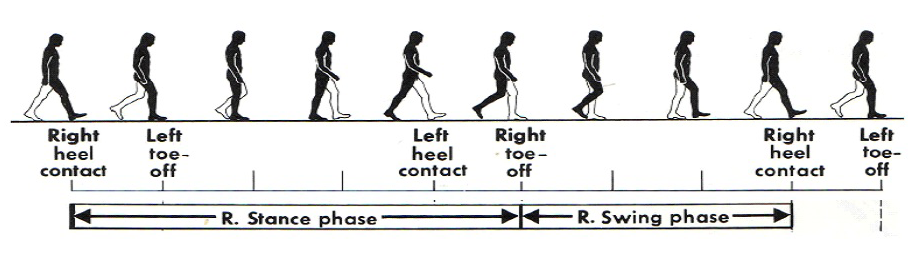
\includegraphics[scale=0.6]{imagenes/apartado_2/221_ciclo_paso_humano}}
\caption{Representación gráfica del paso o caminata}
\label{figura221}
\end{figure}

\newpage

\subsection{Zero Moment Point (ZMP)}

Vukobratović \cite{ref16} fue uno de los primeros en introducir el concepto más importante y principal a la hora de mantener el equilibrio de los robots humanoides bípedos. Decía que durante el paso, aparte de la realización del movimiento relativo entre juntas del mecanismo, la tarea más importante es preservar el equilibrio dinámico. Para ello toda el área del pie (incluyendo sus bordes) debe estar en contacto con el suelo.

\begin{figure}[H]
\centering
{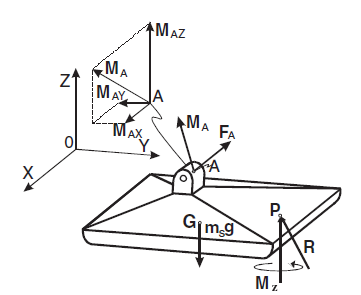
\includegraphics[scale=0.6]{imagenes/apartado_2/222_fuerzas_momentos}}
\caption{Representación de fuerzas y momentos que actúan sobre el pie de apoyo}
\label{figura222}
\end{figure}

Si el mecanismo está en equilibrio quiere decir que en el punto P de la suela, donde actúan las fuerzas de reacción del suelo,

\begin{equation}
\begin{split}
Mx=0\\
My=0
\end{split}
\label{ec21}
\end{equation}

Gracias a ello el punto P pasó a denominarse Punto de Momento Cero (ZMP), pudiéndose reducir dichas fuerzas a una sola llamada $R$ y a la componente z del momento $M_z$ sobre dicho punto.

Para calcular dicho punto y asegurarse de que el mecanismo está en equilibrio dinámico, teniendo en cuenta la dinámica del mecanismo, el requisito indispensable es que el pie esté completamente apoyado en el suelo. Para ello hay que partir de las ecuaciones del equilibrio estático para el pie de apoyo:

%%Ecuaciones 2 y 3
\begin{equation}
R+F_A+m_sg=0
\label{ec22}
\end{equation}
\begin{equation}
\overrightarrow{OP} \times \overrightarrow{R}+\overrightarrow{OG} \times m_sg + M_A+M_Z+\overrightarrow{OA} \times F_A=0
\label{ec23}
\end{equation}

donde $\overrightarrow{OP}$, $\overrightarrow{OG}$ y $\overrightarrow{OA}$ son los vectores desde el origen del sistema de coordenadas $O_(xyz)$ al punto P donde actúan las fuerzas de reacción del suelo, el centro de masas del pie (G), la articulación del tobillo (A), y la masa del pie $m_s$.

Dando su proyección en el plano horizontal se obtiene:

%%aquí va la eq 4.
\begin{equation}
(\overrightarrow{OP} \times \overrightarrow{R})^H+\overrightarrow{OG} \times m_sg+ (M_A)^H+(\overrightarrow{OA} \times F_A)^H=0 
\label{ec24}
\end{equation}

Esta ecuación permite calcular la posición del punto de actuación de la fuerza de reacción del suelo (P) para la dinámica general del mecanismo. Sin embargo esto no sirve para saber si está en equilibrio dinámico cuando el sistema está en movimiento. Para ello hay que tener en cuenta el punto P calculado y el polígono de soporte. Como el punto P calculado con ec \eqref{ec24} nunca puede existir fuera del polígono de soporte, ya que si lo hiciera la fuerza total R no actuaría sobre el sistema, sólo si éste está dentro del polígono de soporte el sistema estará en equilibrio dinámico.

Si suponemos que el punto P obtenido de $M_x=M_y=0$ está fuera del polígono de soporte, consideraríamos dicho punto como ZMP ficticio (\textbf{FZMP}). 

Ésto se puede explicar en el caso en el que el ZMP se está acercando al borde del polígono de soporte (tanto en simple soporte como en doble soporte). Si no hubiera más momentos adicionales, el sistema estaría en equilibrio (ZMP), pero si hay momentos adicionales el mecanismo comenzaría a girar y se colapsaría, ya que el punto de actuación de la fuerza de reacción del suelo estaría al borde del pie. Dicho punto ya no sería el ZMP.

Cuando el mecanismo está en movimiento, una manera de determinar el ZMP es midiendo las fuerzas que actúan cuando el pie entre en contacto con el suelo mediante sensores ubicados en la suela del mecanismo (todos los sensores deben estar en contacto con el suelo, ya que si no se cumple el mecanismo giraría en el borde del pie y volcaría), calculando dicho punto mediante el CoP, que se ha explicado anteriormente . Otra manera sería mediante un modelo dinámico. A partir de las fuerza y el momento en la articulación del tobillo ($F_A$ y $M_A$) el procedimiento para calcular ZMP consta de dos pasos:

\begin{enumerate}
\item Calcular $\overrightarrow{OP}$ de la ec \eqref{ec24}. La posición obtenida de P sería el ZMP. Aquí no sabemos todavía si el punto P se encuentra dentro o fuera del polígono de soporte porque no se tiene en cuenta el tamaño real de dicho polígono (figura \ref{figura223} a).

\item Una vez calculada la posición del ZMP, se compara con el tamaño real del polígono de soporte. Si está fuera significa que que el punto de actuación P de las fuerzas de reacción del suelo se encuentra en el borde del polígono de soporte y se poducirá una rotación del mecanismo debido al momento de desequilibrio, cuya intensidad depende de la distancia entre el borde del polígono de soporte y la posición del ZMP calculada, es decir, a la posición del FZMP. Si se encuentra dentro del polígono, el mecanismo estaría en equilibrio (figura \ref{figura223} b).

\begin{figure}[H]
\centering
\subfigure[]
{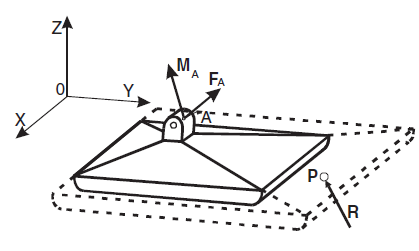
\includegraphics[scale=0.5]{imagenes/apartado_2/223_1_zmp}}
\quad
\subfigure[]
{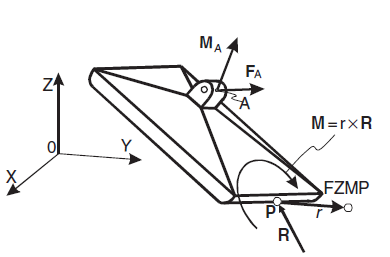
\includegraphics[scale=0.55]{imagenes/apartado_2/223_2_zmp}}
\caption{Determinación del ZMP}
\label{figura223}
\end{figure}

\end{enumerate}

\textbf{RELACIÓN ENTRE ZMP, FZMP Y COP}

Únicamente si la fuerza resultante $R$ está equilibrada con todas las fuerzas activas del sistema bípedo, el CoP y el ZMP coinciden, entonces podríamos decir que se encuentra en equilibrio dinámico, $P \equiv CoP \equiv ZMP$, como se muestra en la figura \ref{figura224}a \cite{ref24}. 

\begin{figure}[H]
\centering
\subfigure[Dinámicamente estable]
{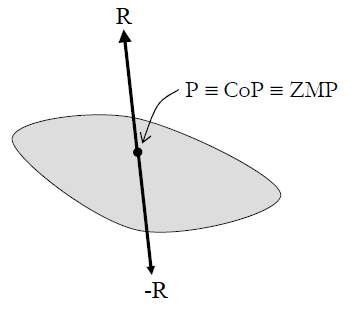
\includegraphics[scale=0.5]{imagenes/apartado_2/224_1_cop_zmp}}
\quad
\subfigure[Dinámicamente inestable]
{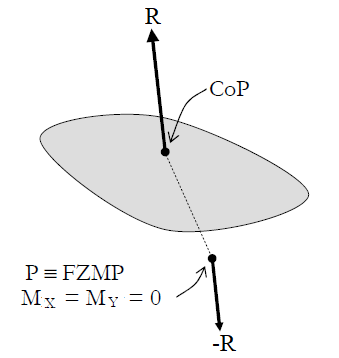
\includegraphics[scale=0.55]{imagenes/apartado_2/224_2_cop_zmp}}
\caption{Relación entre ZMP, FZMP y CoP}
\label{figura224}
\end{figure}

Sin embargo, si nos fijamos en la figura \ref{figura224}b vemos que el punto de ataque de las fuerzas cae fuera del soporte de apoyo, ZMP y CoP no coinciden, por lo que ahora $P \equiv FZMP$.

\afterpage{\null\newpage}
\newpage



\section{Descripción del sistema}

\subsection{Robot humanoide TEO}

El desarrollo del actual proyecto se produjo sobre el robot humanoide de tamaño completo TEO (Task Environment Operator) del grupo de investigación RoboticsLab, en el departamento de Ingeniería de Sistemas y Automática de la Universidad Carlos III de Madrid. Se trata de una versión mejorada de su predecesor Rh-1. Posee 28 grados de libertad y pesa alrededor de 63 kg.

\begin{figure}[H]
\centering
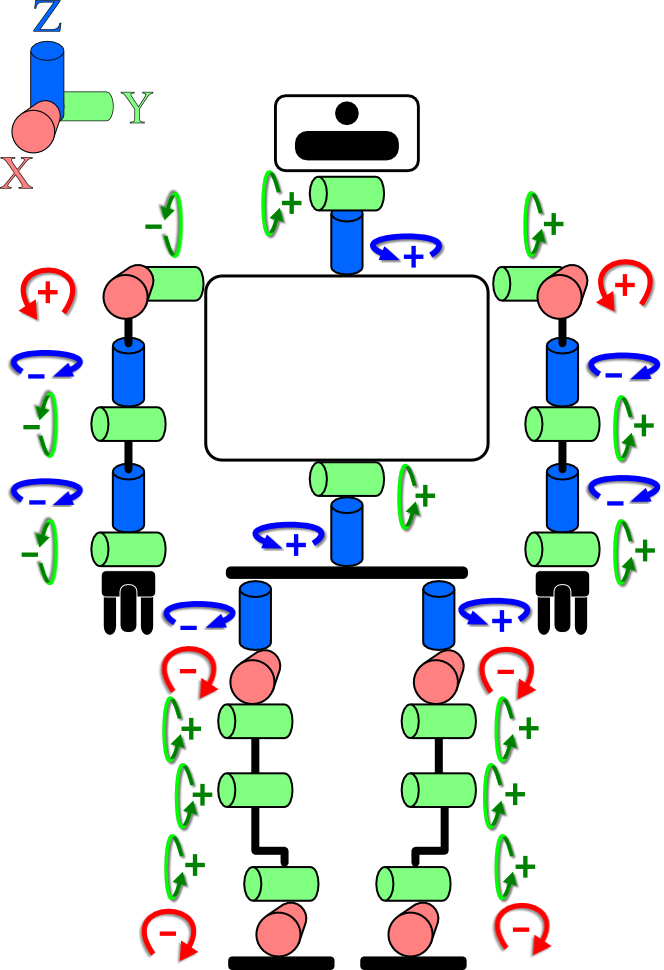
\includegraphics[scale=0.3]{imagenes/apartado_3/31_teo_joints}
\caption{Diagrama articulaciones TEO}
\label{figura31}
\end{figure}

%%Para mirar la pagina de lo que esta compuesto TEO es robot household companion

Está compuesto por varios motores paso a paso que se encargan de mover las articulaciones, 4 sensores de fuerza-par (2 en las muñecas y otros 2 en los tobillos) y un sensor inercial (IMU) que se encargan de recoger toda la información proveniente del entorno, un sistema de visión, realizada a través de una cámara ASUS, y 4 microprocesadores, que se encargan de controlar las principales funciones.

Estos microprocesadores son: visión artificial, que se encarga de computar las imágenes que recibe el robot a través de la cámara; locomoción, encargado de controlar las piernas y la posición del torso, y de obtener la información de los sensores de fuerza-par situados en los tobillos para mantener el robot en equilibrio en todo momento y mantenga una posición erguida, se encuentre en posición estática o caminando.

Para la adquisición de datos, como se ha comentado anteriormente, el robot posee una IMU localizada en el tronco, capaz de medir aceleraciones, campos magnéticos y ángulos,  y 4 sensores de fuerza-par situados en muñecas y tobillos, capaces de medir fuerzas y torques.

En cuanto a la comunicación se usa un protocolo CAN-bus y el software para controlar dichas comunicaciones entre CAN-bus y el ordenador se denomina YARP\footnote{YARP (Yet Another Robot Platform) es un middleware (software que ayuda a una aplicación a interactuar o comunicarse con otras aplicaciones, paquetes de programas, hardware, redes, y/o sistemas operativos) escrito en C ++ para interconectar sensores, procesadores y actuadores en robots.}.

\begin{figure}[H]
\centering
\subfigure[CAN-bus]
{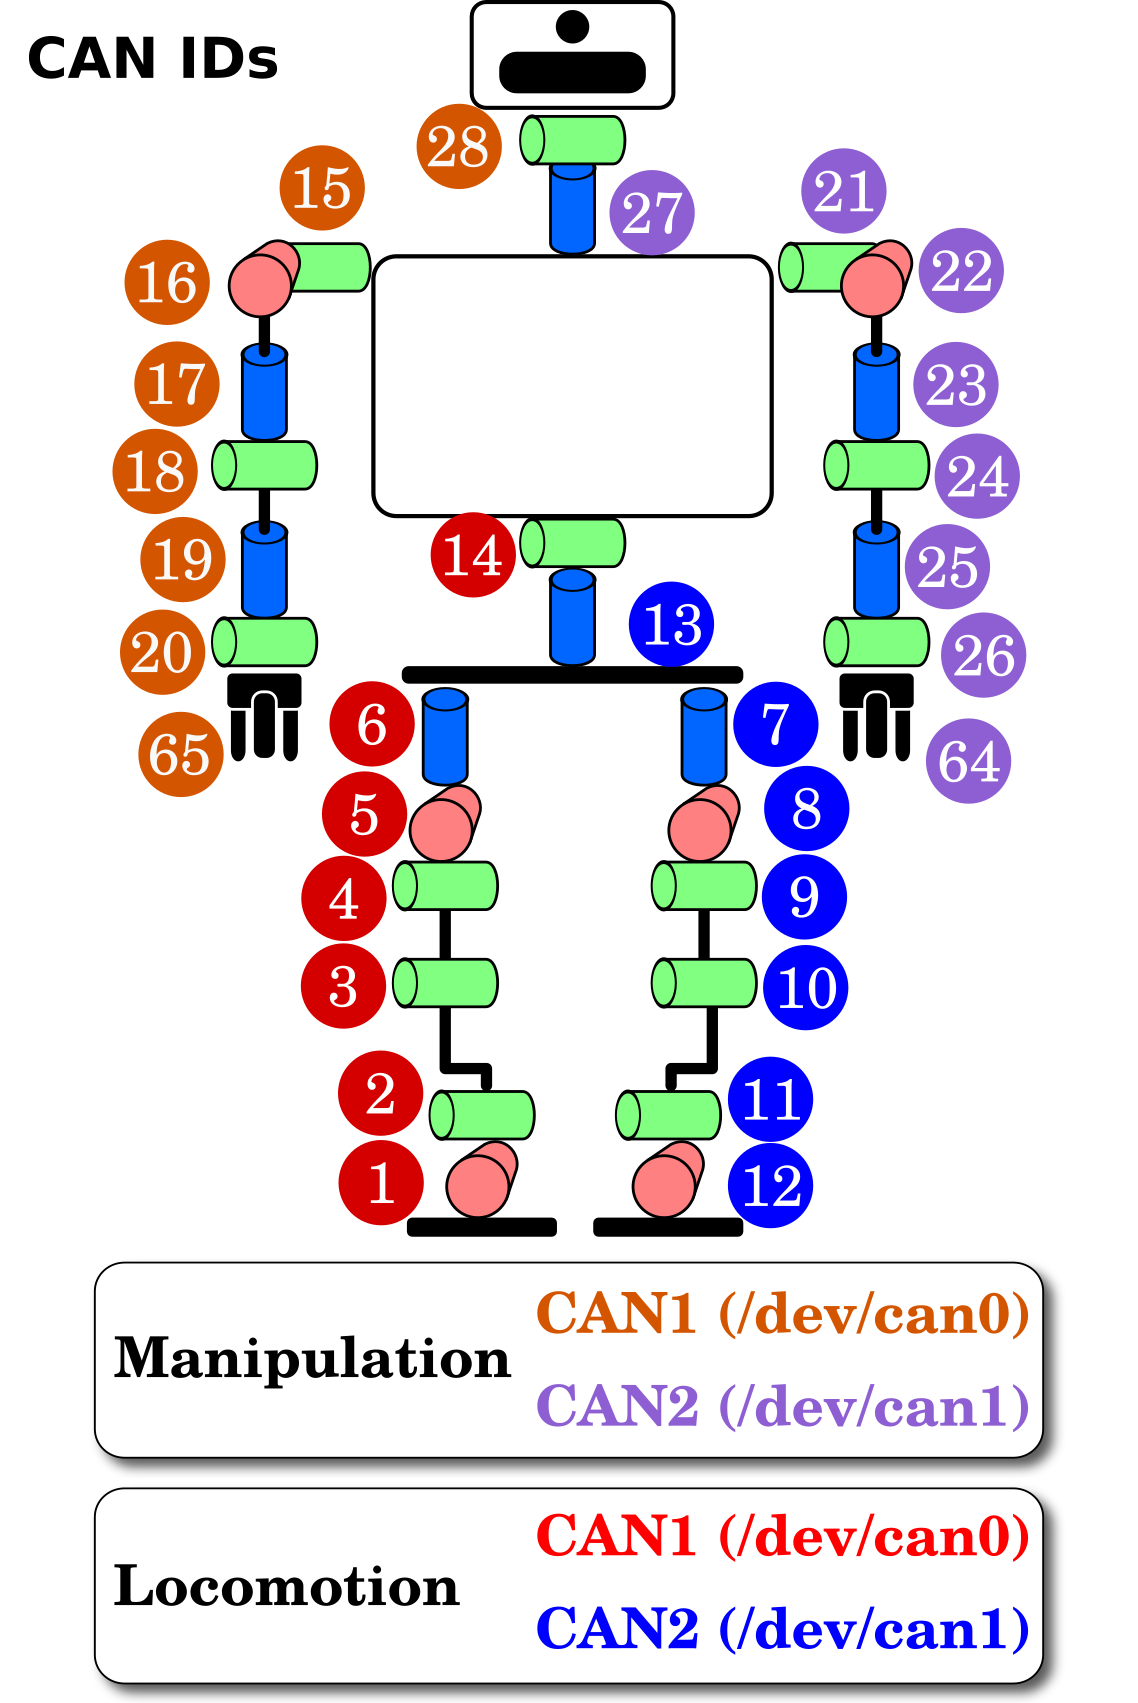
\includegraphics[scale=0.23]{imagenes/apartado_3/32_1_can_bus}}
\quad
\subfigure[YARP]
{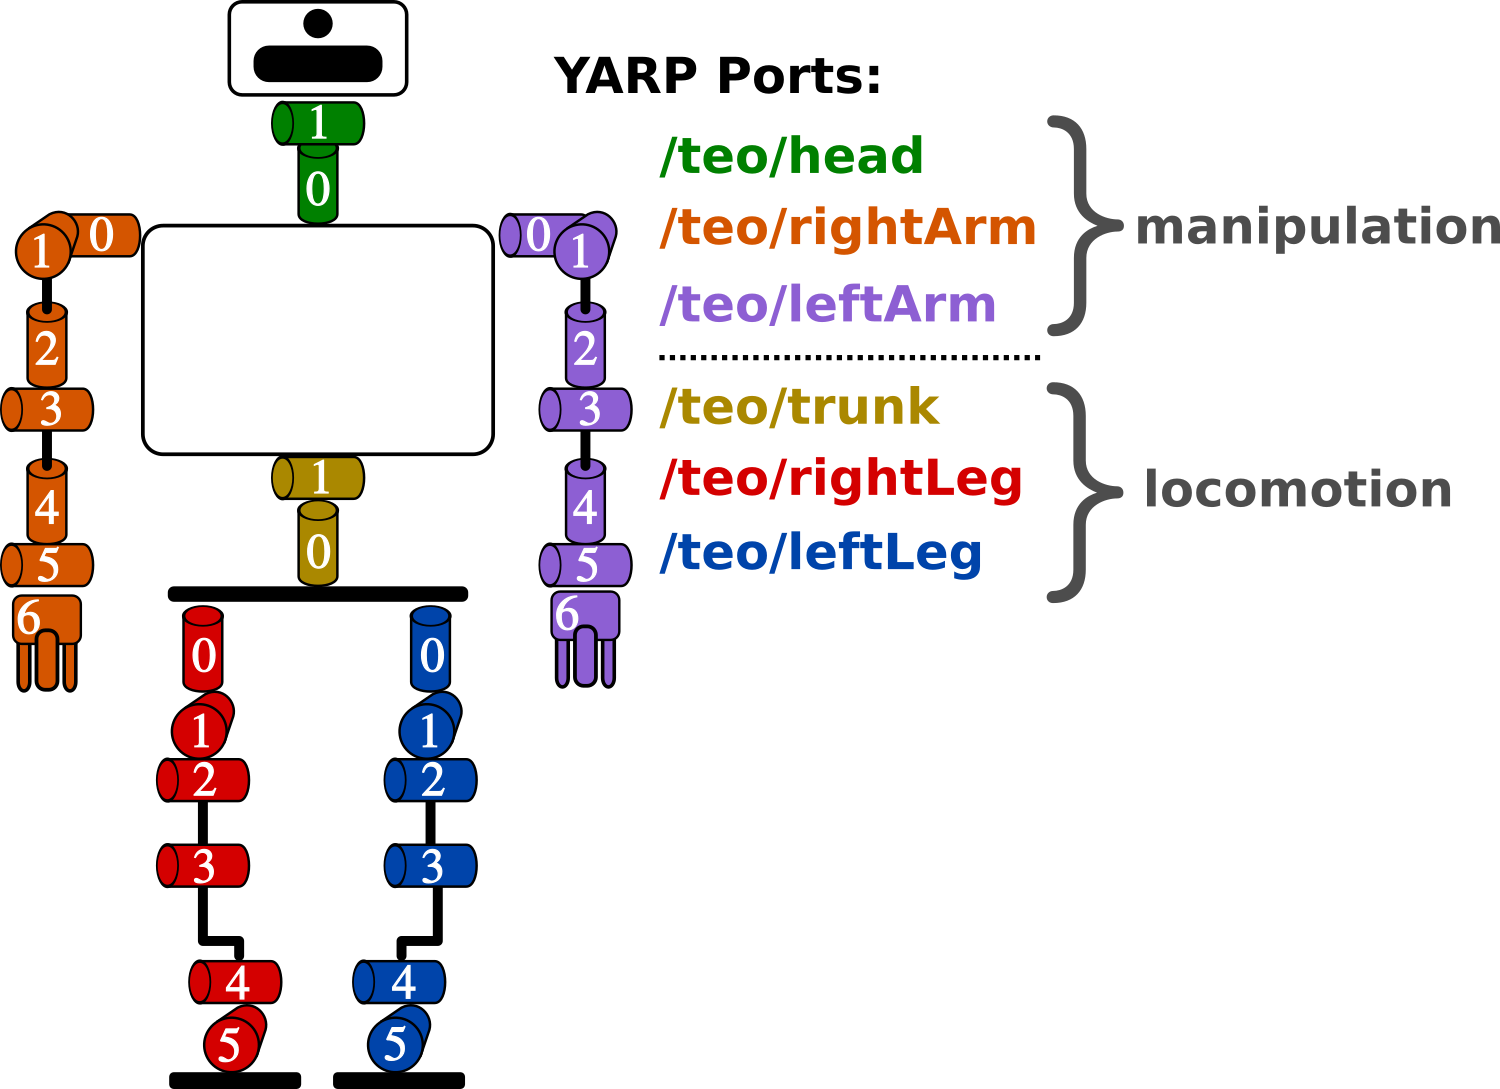
\includegraphics[scale=0.23]{imagenes/apartado_3/32_2_yarp}}
\caption{Esquema comunicaciones TEO}
\label{figura32}
\end{figure}

\begin{figure}[H]
\centering
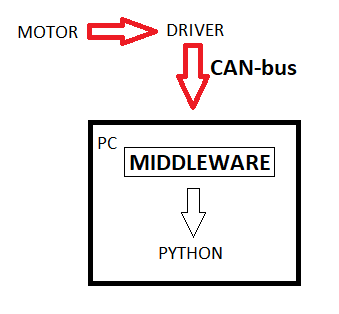
\includegraphics[scale=0.6]{imagenes/apartado_3/33_diagrama_comunicaciones}
\caption{Diagrama comunicaciones con PC}
\label{figura33}
\end{figure}

\subsection{Sensores fuerza-par}

Los sensores fuerza-par son dispositivos mecánicos basados en extensómetros dispuestos de tal manera que permiten obtener medidas de fuerzas y momentos en 3 dimensiones.

\subsubsection{JR3 50M31A y 85M35A}
Los sensores de fuerza-par montados en TEO son sensores proporcionados por la compañía JR3 Inc. y cuyos modelos son 50M31A para las muñecas y 85M35A para los tobillos. Según el fabricante los dos primeros números indican el diámetro de los sensores, seguidos del número de serie, para acabar con dos dígitos que indican su espesor.

Al tratarse de diferentes modelos, éstos poseen diferentes fondos de escala, como se aprecia en la tabla \ref{tabla31}.

\begin{table}[H]
\begin{center}
    \begin{tabular}{| c | c | c | c | c |}
    \hline
    \rowcolor[gray]{0.7} Articulación & Modelo & $F_{x,y}$ & $F_{z}$ & $M_{x,y,z}$ \\ \hline
    \cellcolor[gray]{0.9}Muñeca & 50M31A & 100N & 200N & 5Nm \\ \hline
    \cellcolor[gray]{0.9}Tobillo & 85M35A & 250N & 500N & 212Nm\\ \hline
    \end{tabular}
\end{center}
\caption{Modelos y características de los sensores F-T. [JR3 Inc.]}
\label{tabla31}
\end{table}

Estas diferencias se deben a que los tobillos deben soportar más fuerzas y momentos no sólo producidos por cualquier carga que pueda transportar el robot sino por su propio peso también.

Los sensores de la serie M están compuestos por una serie de elementos electrónicos internos que ayudan a filtrar el ruido, proporcionan una salida digital para usar con una tarjeta PCI, para la adquisición de datos, del mismo fabricante y una salida analógica. En cuanto a su precisión los sensores de esta serie poseen una precisión nominal del 1\% sobre la escala completa.

Para terminar, estos sensores permiten la adquisición de datos en unidades del Sistema Internacional o en unidades del sistema imperial, señalados en la figura \ref{figura34}.

\begin{figure}[H]
\centering
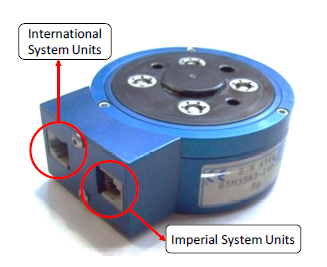
\includegraphics[scale=0.8]{imagenes/apartado_3/34_jr3_sensor}
\caption{Sensor fuerza-par JR3 85M35A}
\label{figura34}
\end{figure}

\subsubsection{Adquisición de datos}

Para la adquisición de datos, como se ha mencionado anteriormente, se utiliza una tarjeta PCI proporcionada por la misma compañía que los sensores JR3 Inc, cuyo modelo es PCI 1592D, compuesta por 4 puertos (nombrados en la figura \ref{figura35}). La tarjeta PCI utiliza cables de 6 u 8 pines (RJ-11 y RJ-45 respectivamente) para recibir datos de alta velocidad de los sensores que se conectan a través de estos cables, y proporcionar alimentación a dichos sensores. Esta tarjeta PCI se encuentra instalada detrás del microprocesador de manipulation en el robot.

\begin{figure}[H]
\centering
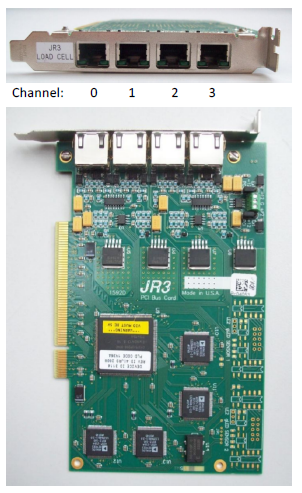
\includegraphics[scale=0.7]{imagenes/apartado_3/35_tarjeta_adquisicion_datos}
\caption{Tarjeta de adquisición de datos \textsl{JR3}}
\label{figura35}
\end{figure}

Para acceder a los datos recibidos de los sensores, es necesario acceder a la dirección de memoria para cada dato disponible de la tarjeta.

Estos datos se pueden obtener en dos tipos de unidades: en unidades del Sistema Internacional o en unidades del Sistema Imperial, por ello hay que estar atentos de qué puerto de los sensores se están obteniendo los datos. En el SI las fuerzas están dadas en Newton [$N$] y los pares en Decanewton por metro [$dN \cdot m$].

\subsubsection{Programa de adquisición de datos}

El programa \textsl{jr3pci4channelYarp}(disponible en https://github.com/roboticslab-uc3m/LoliRepo/tree/master/TFM/jr3Yarp/jr3pci4channelYarp) lee los datos obtenidos de los 4 sensores de fuerza-par del robot TEO.

El tiempo de ciclo del programa es de aproximadamente $20\mu s$ por cada sensor, por lo que los cuatro sensores que leen el tiempo de ciclo es de aproximadamente $80\mu s$.

El conjunto de datos leídos de la tarjeta de adquisición se obtiene en unidades de SI, y se manda a través de puertos YARP mediante un objeto YARP Bottle. Los datos, cuando llegan al cliente, se retrasan entre $10$ y $50\mu s$, dependiendo del ciclo de procesamiento del lector, debido a que hasta que el cliente no finaliza el procesamiento anterior no llegan las actualizaciones de los datos, todo ello para que no se pierdan actualizaciones por parte del cliente \cite{ref14}%%%%%%[yarp].

La figura \ref{figura36} muestra el procedimiento de adquisición de datos, y la figura \ref{figura37} muestra una captura de pantalla del programa en ejecución.


\begin{figure}[H]
\centering
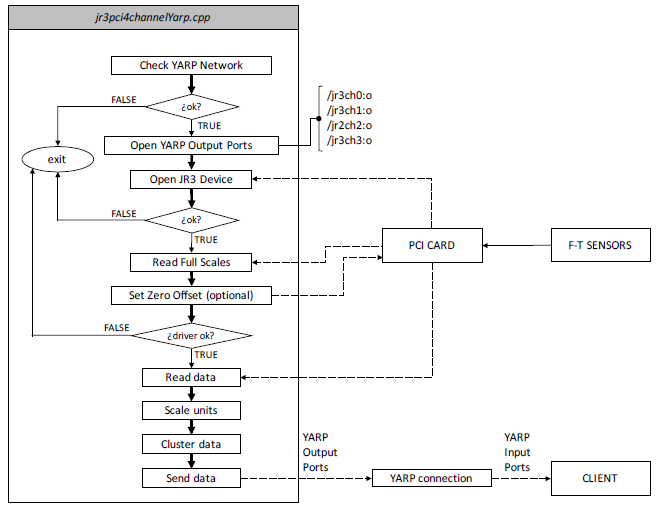
\includegraphics[scale=0.8]{imagenes/apartado_3/36_programa_adquisicion_datos}
\caption{Diagrama comunicaciones con PC}
\label{figura36}
\end{figure}

\newpage

\subsection{Unidad de medida inercial (IMU)}

Para el sistema de percepción como se ha comentado antes se utiliza una IMU, capaz de medir aceleraciones lineales, campos magnéticos y velocidades angulares, gracias a la combinación de acelerómetros, giróscopos y magnetómetros, y en algunos casos incluso barómetros, para obtener información de la temperatura, presión y altitud.

- \emph{Acelerómetro}: Dispositivo que mide el cambio de aceleración o vibración debido a los movimientos de la estructura a la que está acoplado. %%sacado de diversas paginas, poner la primera que aparece al poner acelerometro

- \emph{Giróscopo}: Dispositivo mecánico que sirve para medir cambios de orientación en el espacio tridimensional. %%Sacado de wikipedia

- \emph{Magnetómetro}: Dispositivo que sirve para cuantificar la fuerza o la dirección del campo magnético de un punto en el espacio.

\subsubsection{Xsens MTi-28A53G35}

La unidad montada en el tronco de TEO pertenece al modelo MTi-28A53G35 proporcionado por la compañía Xsens. Se trata de un AHRS (Attitude and Heading Reference System) y a la vez de una IMU de tamaño y peso reducidos con 3 grados de libertad, compuesto por acelerómetros, giróscopos y megnetómetros 3D.

Su procesador interno de baja potencia proporciona una señal de orientación sin derivación(gracias a que utiliza la gravedad y el campo magnético de la tierra como vectores de referencia), aceleración calibrada, giros y datos de campo magnético terrestre, todo ello en 3D.

\begin{figure}[H]
\centering
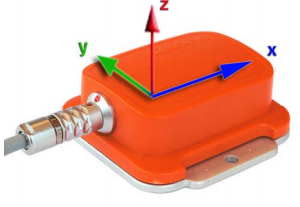
\includegraphics[scale=0.6]{imagenes/apartado_3/37_2_inertial_sensor_xsens}
\caption{IMU}
\label{figura37}
\end{figure}

Su tamaño, peso y consumos reducidos, en adición a su robustez de diseño, lo hacen el sensor ideal para poder acoplar en cualquier dispositivo que requiera mediciones de aceleración, giros o campos magnéticos. 

\newpage

Entre sus caracterísicas más destacadas se encuentran la capacidad de calcular en tiempo real el rumbo y datos dinámicos inerciales, orientación 360º referenciada por la gravedad y el campo magnético de la tierra, alta velocidad de actualización (120 Hz), y calibrado individual para la temperatura, la desalineación 3D y la sensibilidad cruzada del sensor. Además, el MTi incorpora una rutina de mapeado del campo magnético para corregir los efectos del hierro.

\begin{table}[H]
\centering
\begin{tabular}{c|c|}
\cline{2-2}
 & \cellcolor[gray]{0.7}MTi-28A\#\#G\#\# \\ 
 \hline
\multicolumn{1}{|c|}{\cellcolor[gray]{0.9}Interfaz} & \begin{tabular}[c]{@{}c@{}}Digital Serial\\ (RS-232)\end{tabular} \\ 
\hline
\multicolumn{1}{|c|}{\cellcolor[gray]{0.9}\begin{tabular}[c]{@{}c@{}}Voltaje de\\ funcionamiento\end{tabular}} & 4.5-15V \\ 
\hline
\multicolumn{1}{|c|}{\cellcolor[gray]{0.9}\begin{tabular}[c]{@{}c@{}}Consumo de Energía\\ (modo orientación\\ AHRS/3D)\end{tabular}} & 360mW \\ 
\hline
\multicolumn{1}{|c|}{\cellcolor[gray]{0.9}\begin{tabular}[c]{@{}c@{}}Rango de Operación \\ de Temperatura\end{tabular}} & 0ºC - 55ºC \\ 
\hline
\multicolumn{1}{|c|}{\cellcolor[gray]{0.9}\begin{tabular}[c]{@{}c@{}}Dimensiones\\ Exteriores\end{tabular}} & \begin{tabular}[c]{@{}c@{}}58 x 58 x 22 mm\\ (W x L x H)\end{tabular} \\ 
\hline
\multicolumn{1}{|c|}{\cellcolor[gray]{0.9}Peso} & 50g \\ \hline
\end{tabular}
\caption{Características sensor IMU MTi-28A [Xsens]}
\label{tabla32}
\end{table}

Todo los datos recogidos por el sensor MTi son volcados e interpretados por la computadora gracias al MTi SDK (Software Development Kit), un paquete propietario de Xsens que sirve de interfaz a múltiples niveles: librerías binarias API%%abreviatura 
(Windows, Linux), pero también proporciona código fuente implementando el protocolo de comunicación binario MTi para una fácil integración en cualquier plataforma \cite{ref12}.

%%Este apartado sacado de http://www.sensores-de-medida.es/uploads/0referencia_inercial_mti_ahrs.pdf
%%http://wiki.icub.org/images/8/82/XsensMtx.pdf

El software para acceder al sensor incercial MTi, que está instalado en la CPU de locomoción de TEO, se ha extraído del robot iCub\footnote{iCub se trata de un robot humanoide para la investigación en cognición corporal que fue desarrollado entre el Instituto Italiano de Tecnología y la Universidad de Génova, dentro del consorcio internacional RobotCub, en el que participan varias universidades europeas. Mide 104cm de altura, pesa 22kg y posee 53 grados de libertad. Posee sensores de cámara, micrófonos, sensores inerciales, sensores fuerza/par, sensores de posición o sensores táctiles.}, cuyo software es de código abierto siguiendo las licencias GPL/FDL y desarrollado sobre YARP, gracias a que éste tenía implementado el acceso a uno de sus sensores incerciales MTx.

El envío de datos se realiza a través de un cable RS-232 (CA-USB2) que incluye un convertidor a USB, como el de la figura \ref{figura38}.

\begin{figure}[H]
\centering
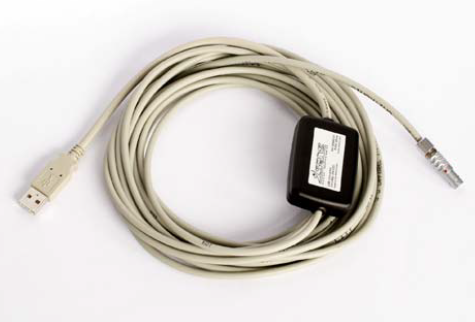
\includegraphics[scale=0.6]{imagenes/apartado_3/38_cable_rs_232}
\caption{Cable \textsl{RS-232}}
\label{figura38}
\end{figure}

\afterpage{\null\newpage}
\newpage
\section{Estudio de la estabilidad}

El control de la estabilidad en los robots bípedos resulta muy complejo. Para solucionarlo muchos investigadores han simplificado el cuerpo del robot. 

En este capítulo se van a explicar las dos simplificaciones más utilizadas a la hora de estudiar la estabilidad de los robots humanoides bípedos, y más en concreto la estabilidad del robot TEO utilizado en el actual proyecto.



\subsection{Modelo Péndulo Invertido Lineal}

La primera de ellas es el modelo del péndulo invertido lineal (LIPM)%%abreviatura.
. Éste es el modelo más básico utilizado para simplificar la cinemática y la dinámica de los robots bípedos. Se trata de un modelo desarrollado en dos dimensiones con uno (una única unión rotacional)o dos (incluyendo una unión lineal) grados de libertad. S. Kajita \cite{ref10} llegó a este modelo haciendo tres suposiciones. La primera de ellas es que la masa total del robot está concentrada en el CoM. En la segunda supone que el robot tiene piernas sin masa, cuyas puntas entran en contacto con el suelo a través de puntos de rotación individuales. Y la última considera que el robot se mueve solamente en el plano sagital (mostrado en la figura \ref{figura41}).

\begin{figure}[H]
\centering
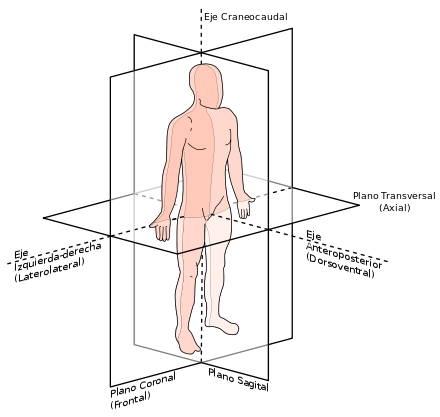
\includegraphics[scale=0.6]{imagenes/apartado_4/41_plano_anatomico_sagital3}
\caption{Planos Anatómicos}
\label{figura41}
\end{figure}

\begin{figure}[H]
\centering
\subfigure[1 grado de libertad]
{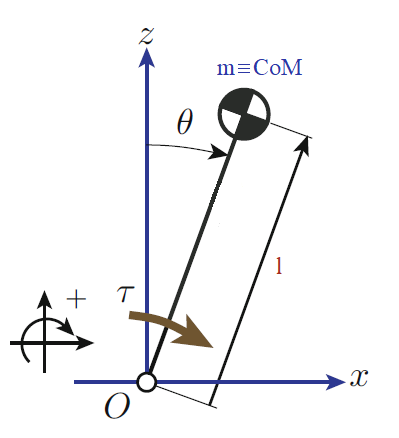
\includegraphics[scale=0.65]{imagenes/apartado_4/42_1_Linear_Inverted_Pendulum_Model_LIPM}}
\quad
\subfigure[2 grados de libertad]
{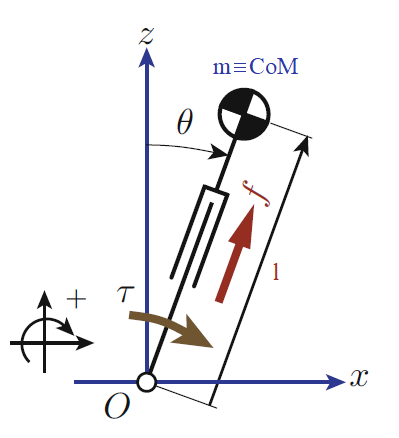
\includegraphics[scale=0.65]{imagenes/apartado_4/42_2_Linear_Inverted_Pendulum_Model_LIPM}}
\caption{Modelo Péndulo Invertido Lineal}
\label{figura42}
\end{figure} 

La ecuación que define el movimiento del CoM es la siguiente:

\begin{equation}
\tau = - ml^2\ddot{\theta}+mgl\sin\theta
\label{ec41}
\end{equation}

donde $m$ es la masa del sistema localizada en el CoM, $l$ es la longitud del péndulo, $\tau$ es el par en el punto de rotación y $\theta$ es el ángulo del péndulo. Sin embargo, esta es una ecuación no lineal, por lo que resulta en un controlador muy complejo para el robot. Para resolver este problema asumimos que $\theta$ es lo suficientemente pequeño ($\theta<10º$) como para considerar que $\sin\theta=\theta$. Esta simplificación le permitió a Kajita desarrollar el modelo más utilizado a lo largo de los años para el estudio de la estabilidad de los robots bípedos, una evolución del modelo lineal en 2D, que le permitió trabajar en 3D, el modelo Péndulo Invertido Lineal en tres dimensiones (3DLIPM%%%%acrónimos)
)\cite{ref15}.

\begin{figure}[H]
\centering
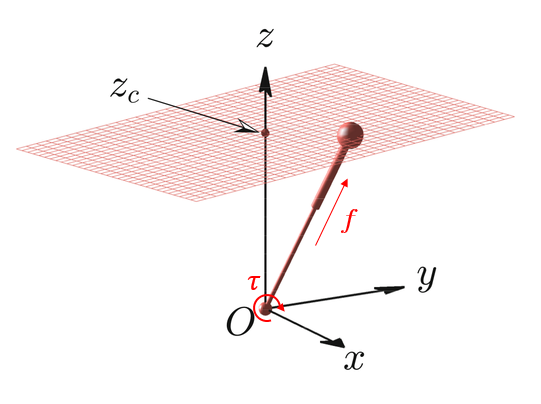
\includegraphics[scale=0.5]{imagenes/apartado_4/43_3D_linear_inverted_pendulum_model}
\caption{Modelo Péndulo Invertido Lineal 3D (3DLIPM)}
\label{figura43}
\end{figure}

Tras la simplificación la ecuación \ref{ec41} queda:

\begin{equation}
\tau = - ml^2\ddot{\theta}+mgl\theta
\label{ec42}
\end{equation}

La posición del CoM $\textbf{p}=(x,y,z)$ está determinada por unas variables de estado $\textbf{q}=(\theta_r,\theta_p,r)$, luego las ecuaciones en los 3 ejes quedan:

\begin{equation}
x=rS_p
\label{ec43}
\end{equation}
\begin{equation}
y=-rS_r
\label{ec44}
\end{equation}
\begin{equation}
z=rD
\label{ec45}
\end{equation}

donde $S_r \equiv \sin\theta_r; S_p \equiv \sin\theta_p; D \equiv \sqrt{1-S_r^{2}-S_p^{2}}$.

Teniendo en cuenta que $(\tau_r,\tau_p,f)$ son los pares y fuerzas asociados a las variables de estado $(\theta_r,\theta_p,r)$, la ecuación del movimiento del péndulo invertido 3D queda descrita matemáticamente como:

\begin{equation}
m\begin{pmatrix}
\ddot{x}\\ 
\ddot{y}\\ 
\ddot{z}
\end{pmatrix}=\left (J^{T} \right )^{-1}\begin{pmatrix}
\tau_r\\ 
\tau_p\\ 
f
\end{pmatrix}+\begin{pmatrix}
0\\ 
0\\ 
-mg
\end{pmatrix}
\label{ec46}
\end{equation}

donde la estructura de la jacobiana es:

\begin{equation}
J=\frac{\partial p}{\partial q}=\begin{pmatrix}
0 & rC_p & S_p\\ 
-rC_r & 0 & -S_r\\ 
-rC_rS_r/D &-rC_pS_p/D  & D
\end{pmatrix}
\label{ec47}
\end{equation}

\begin{equation}
C_r \equiv \cos\theta_r, C_p \equiv \cos\theta_p
\label{ec48}
\end{equation}

\begin{equation}
S_r \equiv \sin\theta_r, S_p \equiv \sin\theta_p
\label{ec49}
\end{equation}

\begin{equation}
D \equiv \sqrt{1-S_r^{2}-S_p^{2}}
\label{ec410}
\end{equation}

Sustituyendo \ref{ec43}, \ref{ec44} y \ref{ec45}, se obtienen las ecuaciones de la dinámica en los ejes $x$, $y$ y $z$

\begin{equation}
m\left ( -z\ddot{y} - y\ddot{z} \right ) = \frac{D}{C_r}\tau_r - mgy
\label{ec411} 
\end{equation}

\begin{equation}
m\left ( -z\ddot{x} - x\ddot{z} \right ) = \frac{D}{C_p}\tau_p - mgx
\label{ec412} 
\end{equation}

\begin{equation}
m\left ( -x\ddot{x} + y\ddot{y} + z\ddot{z} \right ) = rf - mgz
\label{ec413} 
\end{equation}

Pero estas ecuaciones del péndulo invertido son no lineales y demasiado complejas para usarlas en la generación de tareas de caminata. Por esta razón se restringe el movimiento del CoM en la coordenada z al plano $Z_c$, cuyo vector normal es $(k_x,k_y,-1)$ \cite{ref38}.

\begin{equation}
z = k_x x + k_y y + z_c
\label{ec414}
\end{equation}

Si el plano de restricción es horizontal $(k_x=k_y=0)$, la dinámica bajo el control de la restricción están dada por

\begin{equation}
\ddot{x}=\frac{g}{z_c}x - \frac{1}{m z_c}\tau_y
\label{ec415}
\end{equation}

\begin{equation}
\ddot{y}=\frac{g}{z_c}y - \frac{1}{m z_c}\tau_x
\label{ec416}
\end{equation}

\begin{equation}
\ddot{z}=0
\label{ec417}
\end{equation}

En el caso de que el plano de restricción esté inclinado ($k_x=k_y\neq0$), se puede obtener la misma dinámica aplicando una restricción adicional para los pares de entrada,

\begin{equation}
\tau_{x} x + \tau_{y} y = 0
\label{ec418}
\end{equation}

A partir del modelo 3DLIPM junto a la restricción horizontal $(k_x=k_y=0)$ podemos obtener la posición de la proyección del Punto de Momento Cero (ZMP) en el suelo \cite{ref33},

\begin{equation}
x_{ZMP} = -\frac{\tau_y}{mg}
\label{ec419}
\end{equation}

\begin{equation}
y_{ZMP} = -\frac{\tau_x}{mg}
\label{ec420}
\end{equation}

\subsubsection{LIPM aplicado al robot humanoide TEO}

Los sensores que se han utilizado son los F-T de los tobillos, ya que son los que están en contacto con el suelo. Gracias a su información se puede calcular la posición del ZMP para que TEO pueda conservar el equilibrio, a partir de las ecuaciones del modelo de péndulo invertido 3DLIPM. 

Las ecs. \ref{ec419} y \ref{ec420} del ZMP para este modelo responden a la ecuación general:

\begin{equation}
x_{ZMP}=-\frac{\sum x\cdot F_z}{\sum F_z}
\label{ec421}
\end{equation}

Pero este modelo se ha tenido que modificar para el robot TEO utilizado en el actual proyecto, ya que se considera que cuando un robot bípedo está soportando su peso en un pie, el tobillo del robot se convierte en el punto pivotante del modelo conectado al CoM del robot a través de su pierna sin masa. Pero este punto pivotante no se encuentra totalmente en el suelo ya que la estructura de TEO está construida de tal manera que el tobillo está elevado respecto al suelo debido a la anchura de la suela del robot, como se muestra en la figura \ref{figura51}. Por lo tanto, la ecuación del ZMP adaptada sería \cite{ref21}:

\begin{equation}
x_{ZMP}=-\frac{\tau_y + h F_x}{F_z}
\label{ec422}
\end{equation}

donde $\tau_y$ es el par en el punto pivotante alrededor del eje $y$, $F_x$ y $F_z$ son las fuerzas medidas en las direcciones $x$ y $z$ respectivamente, y $h$ es la altura de la suela del robot hasta la localización del sensor F-T.

\begin{figure}[H]
\centering
\includegraphics[scale=0.8]{imagenes/apartado_4/44_LIPM_TEO}
\caption{Modelo LIPM con un sensor F-T entre el tobillo y la suela \cite{ref26}}
\label{figura44}
\end{figure}

Pero esta ecuación sólo valdría cuando el robot está apoyado sobre una pierna (simple apoyo). Sin embargo, el proyecto se ha desarrollado estando apoyadas las dos piernas (doble apoyo), por lo que la ecuación para el ZMP global es:


\begin{equation}
x_{ZMP_{DS}}=\frac{x_{ZMP}^{R}F_{z}^{R}+x_{ZMP}^{L}F_{z}^{L}}{F_{z}^{R}+F_{z}^{L}}
\label{ec423}
\end{equation}

donde R indica la pierna derecha y L la pierna izquierda. A pesar de que en doble apoyo el robot tiene dos puntos pivotantes en los tobillos, se puede aplicar el modelo de péndulo invertido simple ya que ambos tobillos tienen el mismo movimiento a lo largo del eje $x$ (plano sagital).

\subsubsection{DLIPM: mejora del modelo del péndulo invertido simple}\label{definicionDLIPM}

En la respuesta dinámica del modelo de péndulo invertido simple se observaba que había cierto error conforme se aumentaba el ZMP. Ésto se corrigió en \cite{ref21} con una mejora de dicho modelo en la respuesta dinámica eliminando ese error, es decir, ajustando el ZMP calculado a partir de los datos obtenidos de los sensores F-T de los tobillos a un ZMP teórico al que debería llegar el robot. Este modelo se denomina DLIPM.

\begin{figure}[H]
\centering
\includegraphics[scale=0.45]{imagenes/apartado_4/45_modelo_dlipm}
\caption{Modelo DLIPM}
\label{figura45}
\end{figure}

Esta mejora consiste en la adición de un muelle $k_a$ y un amortiguador $B_a$ (figura \ref{figura45}) para compensar la respuesta del estado estacionario ($k_a$) y la respuesta del régimen transitorio para limitar las oscilaciones ($B_a$) del sistema LIPM.

La ecuación del movimiento de dicho modelo estaría dada por:

\begin{equation}
\tau = -ml\ddot{x}(t) - B_a l\dot{x}(t) - k_a lx(t) + mgx(t)
\label{ec424}
\end{equation}

donde $x(t)$ indica el movimiento del CoM, $m$ es la masa del péndulo localizada en el CoM, $l$ la longitud del péndulo, $k_a$ la constante del muelle y $B_a$ la constante del amortiguador. El desplazamiento del CoM es tan pequeño que se puede asumir que $\sin\theta = \theta$, quedando la ecuación 4.24 como:

\begin{equation}
\tau = -ml\ddot{\theta}(t) - B_a l\dot{\theta}(t) - k_a l\theta(t) + mg\theta(t)
\label{ec425}
\end{equation}

Por otra parte, el par también se puede obtener de la medición del ZMP como:

\begin{equation}
\tau = - x_{FT} \cdot mg
\label{ec426}
\end{equation}

donde $x_{FT}$ es la coordenada x del ZMP medido por los sensores de los tobillos. Combinando \ref{ec425} y \ref{ec426} se obtiene:

\begin{equation}
- x_{FT} \cdot mg = -ml\ddot{\theta}(t) - B_a l\dot{\theta}(t) - k_a l\theta(t) + mg\theta(t)
\label{ec427}
\end{equation}

Siendo ésta la ecuación que explica la física del modelo DLIPM que se ha desarrollado en el actual proyecto.

\newpage

\subsection{Modelo cart-table}

La siguiente simplificación más utilizada para el control del equilibrio de los robots humanoides bípedos es el modelo cart-table.

Este modelo proporciona información de las aceleraciones e inercias del cuerpo del robot, muy útiles a la hora de realizar tareas de caminata dinámica. Consiste en un carro de masa M corriendo sobre una mesa sin masa (figura \ref{figura46}). Tiene la misma dinámica de movimiento que el modelo de péndulo invertido pero añade una relación directa entre el ZMP y el movimiento.

\begin{figure}[H]
\centering
\includegraphics[scale=0.5]{imagenes/apartado_4/46_cart_table_model_2}
\caption{Modelo Cart-Table}
\label{figura46}
\end{figure}

Las ecuaciones del modelo cart-table para controlar el ZMP se obtienen sustituyendo \ref{ec419} y \ref{ec420} en \ref{ec415} y \ref{ec416} del modelo 3DLIPM,

\begin{equation}
\ddot{x}_{CoM}=\frac{g}{z_{CoM}}\left ( x_{CoM} - x_{ZMP} \right )\Rightarrow x_{ZMP} = x-\frac{z_{CoM}}{g}\ddot{x}_{CoM}
\label{ec430}
\end{equation}

\begin{equation}
\ddot{y}_{CoM}=\frac{g}{z_{CoM}}\left ( y_{CoM} - y_{ZMP} \right )\Rightarrow y_{ZMP} = y-\frac{z_{CoM}}{g}\ddot{y}_{CoM}
\label{ec431}
\end{equation}

Estas ecuaciones se denominan \textbf{Ecuaciones del ZMP}. 

Como se puede observar el pie de la mesa es demasiado pequeño para que el carro permanezca en el borde, por lo que el carro debe llevar una determinada aceleración para que la mesa se mantenga en posición vertical durante un tiempo, en el que el ZMP exista dentro del pie de dicha mesa.

Por otro lado Shuuji Kajita y Bernard Espiau \cite{ref20} añadieron que si esta aceleración es demasiado grande, el ZMP calculado se sale del polígono de soporte (\ref{figura46}a). Esto es porque \ref{ec430} y \ref{ec431} no tienen en cuenta el polígono de soporte ni la restricción unilateral (por lo que se asume que el pie está pegado al suelo, y esto no puede ser viable ya que el robot necesita levantar el pie para caminar). Por ello, hay que tener en cuenta dicha restricción, y como se puede observar en la \ref{figura46}b, la mesa ya no está en vertical, por lo que hay que tener en cuenta la aceleración en z a parte de la gravedad, quedando la ecuación del ZMP como:

\begin{equation}
\ddot{x}_{CoM}=\frac{g}{z_{CoM}}\left ( x_{CoM} - x_{ZMP} \right )\Rightarrow x_{ZMP} = x-\frac{z_{CoM}}{g+\ddot{z}_{CoM}}\ddot{x}_{CoM}
\label{ec432}
\end{equation}

que da el cálculo del ZMP en el borde del polígono de soporte (pie de la mesa). 

\begin{figure}[H]
\centering
\includegraphics[scale=0.6]{imagenes/apartado_4/47_cart_table_real}
\caption{Cálculo del ZMP. a) Modelo ficticio, b) Modelo real}
\label{figura47}
\end{figure}

Esto es importante ya que un ZMP fuera del polígono de soporte implica que el robot podría no mantener el total contacto pie-suelo y la caminata no se produjese según lo planeado. Cuando el ZMP está dentro del polígono de soporte se puede garantizar el contacto total pie-suelo.

\newpage

\subsection{Equivalencia de modelos}\label{equivalencia_modelos}

Para ambos modelos la variable más importante y que tienen en común es la altura del CoM, desde el punto de medida de las fuerzas y los pares para el caso del modelo LIPM (longitud del péndulo), y la longitud desde el suelo hasta el CoM para el modelo cart-table ($Z_{CoM}$). Gracias a que la altura del CoM es común en los dos modelos se ha podido desarrollar una equivalencia entre ambos en el actual proyecto.

Esta equivalencia se ha desarrollado tomando como referencia el modelo LIPM (incluyendo sus mejoras), ya que era el modelo que más se acercaba al ZMP deseado en las pruebas realizadas, y a partir del mismo se despejó la altura del CoM del modelo cart-table. 

Para cualquier instante t durante el paso o en posición estática, los ZMP de ambos modelos coinciden,

\begin{equation}
X_{ZMP_{FT_t}} = X_{ZMP_{IMU_t}} \Leftrightarrow   X_{ZMP_{FT_{(t+1)}}}=X_{ZMP_{IMU_{(t+1)}}}
\label{ec433}
\end{equation}

Por lo tanto:

\begin{equation}
ZMP_{F-T}=ZMP_{IMU}
\label{ec434}
\end{equation}

\begin{equation}
\left.\begin{matrix}
\left.\begin{matrix}
-\frac{\tau+ h F_{x}}{F_{z}}
\end{matrix}\right|_{SS}=X_{CoM}-\frac{Z_{CoM}}{g+\ddot{z}_{CoM}}\ddot{x}_{CoM}
\\ 
\\
\left.\begin{matrix}
\frac{x_{ZMP}^{R}F_{z}^{R}+x_{ZMP}^{L}F_{z}^{L}}{F_{z}^{R}+F_{z}^{L}}
\end{matrix}\right|_{DS}=X_{CoM}-\frac{Z_{CoM}}{g+\ddot{z}_{CoM}}\ddot{x}_{CoM}
\end{matrix}\right\}
\label{ec435}
\end{equation}

donde $x_{CoM}=0$ ya que la referencia del sistema de coordenadas del modelo cart-table siempre es la misma, y por tanto $z_{CoM}$ es constante en todo momento. Como se puede observar el modelo LIPM es equivalente al modelo cart-table tanto en doble como en simple apoyo.

\begin{equation}
x_{ZMP_{F-T}}=-\frac{Z_{CoM}}{g+\ddot{z}_{CoM}}\ddot{x}_{CoM}
\label{ec436}
\end{equation}

Despejando la altura del modelo cart-table e igualando al ZMP del modelo LIPM para que ambos dieran la misma salida de ZMP, ésta quedaría:

\begin{equation}
Z_{CoM}=-\frac{x_{ZMP_{F-T}}(g+\ddot{z}_{CoM})}{\ddot{x}_{CoM}}
\label{ec437}
\end{equation}

\newpage

\subsection{Estrategias de control}

Los seres humanos son capaces de mantener el equilibrio en entornos complejos y novedosos ante diferentes perturbaciones mediante el movimiento de las diferentes partes de su cuerpo. Esta capacidad de respuesta ante perturbaciones externas ha hecho que diferentes investigadores acerquen el estudio de la estabilidad de los seres humanos a los robots humanoides.

Pueden aparecer diferentes perturbaciones que alteren el equilibrio del robot cuando éste se encuentra en una postura estable. Estas perturbaciones pueden aparecer en el plano sagital (perturbaciones anterior-posteriores) o en el plano frontal (perturbaciones mediolaterales). Se han hecho numerosos estudio del equilibrio cuando el robot se encuentra en posición estática, apareciendo diferentes estrategias de control para mantener dicho equilibrio ante la aparición de diferentes perturbaciones. Dichas estrategias se han separado en función de la magnitud de dicha perturbación y de la posición de la postura del robot en: estrategias de tobillo, cadera y paso \cite{ref17} \cite{ref18}.

Estas estrategias están basadas en la cuantificación del cambio de dirección del CoP en las direcciones anteriormente mencionadas.

\begin{figure}[H]
\centering
\includegraphics[scale=0.8]{imagenes/apartado_4/49_balance_strategies}
\caption{Estrategias de balance}
\label{figura49}
\end{figure}

La primera de ellas es la estrategia de tobillo. Ésta se aplica para pequeñas perturbaciones anterior-posteriores que tienen lugar en el plano sagital. Se usa para controlar y mantener el CoP en el polígono de soporte. Cuando ocurre una alteración del equilibrio de baja magnitud el cuerpo del robot se puede considerar como un péndulo invertido ajustándose dicho equilibrio mediante el par de la articulación del tobillo. 

En la estrategia de la cadera, al igual que en la estrategia de tobillo, se actúa en el plano sagital y se basa en el balance del CMP. Ésta interviene cuando la perturbación del equilibrio es lo suficientemente intensa como para que la estrategia del tobillo no sea suficiente. Se utiliza la articulación de la cadera y se puede usar independientemente o en combinación con la estrategia del tobillo. 

La última estrategia es la del paso. Ésta se lleva a cabo cuando aparece una perturbación en la que una aplicación de par contraria en las articulaciones no es suficiente para recuperar el equilibrio. Cuando se realiza el paso el área del polígono de soporte se reajusta, creando unos nuevos límites de equilibrio.

Todas ellas dependen de diferentes factores como puede ser las condiciones del entorno (entornos rocosos o lisos, por ejemplo), la forma de la suela del robot, la altura del cuerpo, o la posición en la que se encuentre en el momento en el que se produce dicha perturbación.


\afterpage{\null\newpage}
\newpage
\section{Estudio de la respuesta de los sensores del robot humanoide TEO y la aplicación de su información al control del equilibrio}

En este capítulo se van a exponer las respuestas de los sistemas sensoriales del robot humanoide TEO a diferentes inclinaciones  para simular perturbaciones pequeñas que cambian la posición del ZMP y mantener el equilibrio del robot haciendo uso de la estrategia de control de los tobillos. Para ello se decidió ajustar un modelo (el modelo de péndulo invertido lineal) de los dos actuales existentes y a partir de él ajustar el otro (el modelo cart-table).

\subsection{Estudio de la respuesta de los sensores F-T}

Para estudiar la respuesta de los sensores F-T ante perturbaciones y aplicar dicha información obtenida al modelo LIPM, y poder así desarrollar un nuevo modelo personalizado, se ha seguido una serie de pasos divididos en tres fases: fase experimental, fase de análisis de datos y fase de validación de resultados, que se ilustran en la figura \ref{figura51}. 

\begin{figure}[H]
\centering
\includegraphics[scale=0.5]{imagenes/apartado_5/51_diagrama_desarrollo_nuevo_modelo}
\caption{Diagrama del desarrollo experimental del nuevo modelo}
\label{figura51}
\end{figure}

\subsubsection{Descripción de la metodología experimental}

Los experimentos han seguido una serie de pasos para que las lecturas fueran correctas. Éstos se dividen en:

NOTA: Los primeros 2 pasos deben realizarse con el robot en suspensión, es decir, sin que toque el suelo con la suela de los pies. A continuación se explicará el motivo.

\begin{enumerate}

\item \textbf{Puesta del robot en posición inicial (Homeposs)}\\ Una vez se ha encendido el robot y las CPU's se va a proceder a la puesta a cero de la posición del mismo, ya que puede haber modificaciones en su posición de anteriores experimentos o simplemente para asegurarse que los experimentos salen correctamente y siempre empiezan desde la misma posición de inicio. Esto debe realizarse con el robot en suspensión para evitar posibles colisiones de los pies con el suelo.

\item \textbf{Corrección offset sensores F-T}\\ Siguiendo con el robot en suspensión y una vez realizada la posición de inicio, desde una terminal se deben iniciar los sensores F-T de los tobillos que se van a encargar de dar la información de las fuerzas y los pares al programa para así poder realizar los experimentos y eliminar los posibles offset que puedan tener los mismos. Es importante que no esté apoyado en el suelo para que cuando se ejecute esta corrección, no se elimine el valor de la fuerza ejercida por la masa del robot. Una vez que se han iniciado los sensores F-T de los tobillos ya se podría bajar el robot para que éstos puedan tener en cuenta su propio peso y las demás fuerzas y pares. 

\item \textbf{Puesta en funcionamiento del programa}\\ Cuando se inicia el programa, existe una primera fase en la que el robot no realiza ningún movimiento. Esto se debe a que se está configurando de tal manera que se elimine el offset que pueda haber al inicio debido a la posición de homeposs del robot, ya que ésta no es perfecta y, debido a la flexibilidad de la estructura y otros errores acumulados, puede no estar totalmente erguido y que las fuerzas en el plano axial no sean cero. 

Una vez que ha pasado esta fase, y estamos seguros de que ese offset se ha eliminado en la medida de lo posible, se envía al robot un $ZMP_{ref}$ \footnote{ZMP de referencia al que el robot debería llegar atendiendo a la física y cálculos teóricos del modelo LIPM} y TEO comanda un ángulo, que ha calculado a partir de la conversión del $ZMP_{ref}$, activando los motores de sus tobillos (inclinando el robot para simular el empuje) y calculando el $ZMP_{F-T}$ del modelo de péndulo invertido lineal hasta que este $ZMP_{F-T}$ se estabiliza, para hacer coincidir tanto la parte transitoria como la parte de régimen permanente del $ZMP_{F-T}$ con el del $ZMP_{ref}$.

\end{enumerate}

\begin{figure}[H]
\centering
\includegraphics[scale=0.5]{imagenes/apartado_5/52_diagrama_flujo1}
\caption{Diagrama de flujo del programa}
\label{figura52}
\end{figure}


\subsubsection{Respuesta del sistema LIPM}

Se realizaron las pruebas sometiendo al robot a una serie de variaciones en el ángulo de los tobillos para simular perturbaciones pequeñas (empujes), con la excepción de que no volvía al ZMP inicial, para así poder modelar mejor la diferencia entre el ZMP esperado y el medido, estudiándose también su variación dinámica a lo largo del proceso. 

En el presente proyecto se ha llevado a cabo una batería de 30 experimentos en el plano sagital (x-z), representado en la figura \ref{figura53}. Esta metodología también se podría aplicar para cualquier otro plano espacial ya que se obtuvieron resultados similares en el plano frontal (y-z).

\begin{figure}[H]
\centering
\includegraphics[scale=0.65]{imagenes/apartado_5/53_postura_inicial_experimental_teo}
\caption{Plano de desarrollo de los experimentos del robot TEO}
\label{figura53}
\end{figure}

La arquitectura de control utilizada en los primeros experimentos seguía el siguiente esquema:

\begin{figure}[H]
\centering
\includegraphics[scale=2.2]{imagenes/apartado_5/54_esquema_bucle_abierto}
\caption{Arquitectura de control de posición básica de ZMP para el modelo LIPM}
\label{figura54}
\end{figure}


En ellos se ajustó la altura del CoM del modelo para reducir lo máximo posible la diferencia entre el ZMP calculado de los F-T y el ZMP deseado. Esta evolución se puede observar de la figura \ref{figura55}, en la que se mejoró la respuesta del sistema pero en la que todavía se mostraba un error en régimen permanente. Como se puede observar, a mayor ZMP el ángulo de inclinación es mayor y el robot es más inestable debido a que éste se encuentra más cerca del borde del polígono de soporte, y los errores tienen mayor influencia, principalmente los que tienen que ver con la flexibilidad de la estructura del robot y sus tolerancias mecánicas. Estos errores se pueden ver en el régimen permanente de la figura \ref{figura55} b). También se observa una oscilación inicial muy grande, algo que se tiene que evitar sobre todo cuando el ZMP se encuentra en el borde del polígono de apoyo. 

\begin{figure}[H]
\centering
\subfigure[altura no ajustada]{\includegraphics[width=7cm, height=6cm]{imagenes/apartado_5/test6_ft}}
\quad
\subfigure[altura ajustada]{\includegraphics[width=7cm, height=5.9cm]{imagenes/apartado_5/55_2_altura_ajustada.pdf}}
\caption{Evolucion ZMP modelo LIPM}
\label{figura55}
\end{figure}

En los siguientes experimentos, cuya arquitectura de control se muestra en la figura \ref{figura56}, se programó un controlador en ZMP para mejorar la respuesta del sistema y reducir el error tanto en régimen permanente como en el transitorio. Se fueron ajustando diferentes variables de dicho controlador, mostrados en la tabla \ref{tabla51}, para comprobar si el $ZMP_{F-T}$ mejoraba su respuesta tanto en estado estático como en el estado transitorio. 

\begin{figure}[H]
\centering
\includegraphics[scale=0.6]{imagenes/apartado_5/56_esquema_bucle_cerrado}
\caption{Arquitectura de control de ZMP mediante controlador PD}
\label{figura56}
\end{figure}


\begin{table}[H]
\begin{center}
\begin{tabular}{|c|c|c|c|}
\hline
Exp. & $k_p$   & $k_d$    & $k_u$ \\ \hline
1    & -0.0025 & 0.00005  & 1    \\ \hline
2    & -0.0025 & 0.00005  & 1.2  \\ \hline
3    & -0.0025 & 0.00005  & 1.4  \\ \hline
4    & -0.0025 & 0.00005  & 2    \\ \hline
5    & -0.005  & 0.0005   & 1    \\ \hline
6    & -0.005  & 0.0005   & 1.65 \\ \hline
7    & -0.01   & 0.0005   & 1    \\ \hline
8    & -0.01   & 0.0005   & 1.65 \\ \hline
9    & -0.05   & 0.005    & 1.65 \\ \hline
10   & -0.015  & -0.00025 & 1.4  \\ \hline
11   & -0.035  & -0.0001  & 1.4  \\ \hline
\end{tabular}
\end{center}
\caption{Batería de experimentos}
\label{tabla51}
\end{table}

\begin{figure}[H]
\centering
\subfigure[Experimento 1]
{\includegraphics[scale=0.2]{imagenes/apartado_5/57_1_exp1}}
\quad
\subfigure[Experimento 3]
{\includegraphics[scale=0.2]{imagenes/apartado_5/57_2_exp3}}
\quad
\subfigure[Experimento 5]
{\includegraphics[scale=0.2]{imagenes/apartado_5/57_3_exp5}}
\quad
\subfigure[Experimento 10]
{\includegraphics[scale=0.2]{imagenes/apartado_5/57_4_exp10}}
\quad
\subfigure[Experimento 11]
{\includegraphics[scale=0.2]{imagenes/apartado_5/57_5_exp11}}
\caption{Evolución ZMP para ZMPref = 5mm}
\label{figura57}
\end{figure}
 

En las pruebas representadas en la figura \ref{figura57}, cuando se lograba ajustar la respuesta en régimen permanente, reduciendo el error entre el $ZMP_{F-T}$ y el ZMP deseado, el régimen transitorio tenía una oscilación muy grande, y como se ha comentado antes esto se tiene que evitar sobre todo en ZMP situados en el borde del polígono de soporte. Por el contrario si se lograba hacer la oscilación inicial un poco más pequeña el tiempo de estabilización del sistema era mayor, por lo que éste se volvía más lento y no se lograba reducir el error del régimen permanente. Es por ello que se hace necesario la mejora del modelo LIPM, tanto para eliminar el error de régimen permanente como para reducir la oscilación y el sobrepaso del régimen transitorio.

\subsubsection{Respuesta del modelo mejorado DLIPM}

Como se ha explicado en el apartado \ref{definicionDLIPM}, se ha aplicado una mejora al modelo LIPM que permitía ajustar de manera dinámica la respuesta del sistema.

Aplicando Laplace a la ecuación de la física del movimiento del nuevo modelo, la función de transferencia quedaría:

\begin{equation*}
-ml{\theta}(S)S^{2} - B_a l{\theta}(S)S - k_a l\theta(S) + mg\theta(S)=- X(S) \cdot mg
\end{equation*}

\begin{equation*}
{\theta}(S)[-ml^{2}S^{2} - B_a lS + (-k_a l + mg)]=- X(S) \cdot mg
\end{equation*}

\begin{equation*}
\frac{{\theta}(S)}{X(S)}=\frac{-mg}{-ml^{2}S^{2} - S B_a l + (-k_a l + mg)}
\end{equation*}

\begin{equation}
\frac{{\theta}(S)}{X(S)}=\frac{\frac{g}{l^{2}}}{S^{2} - S (\frac{B_a}{ml}) + (\frac{k_a}{ml} - \frac{g}{l})}
\label{ec51}
\end{equation}

donde $\gamma=g/l^{2}$, $\alpha=B_{a}/ml$ y $\beta=(k_{a}/ml) - (g/l)$, quedando simplificada:

\begin{equation}
\frac{\theta(S)}{X(S)}=\frac{\gamma}{S^{2}+\alpha S+\beta }
\label{ec52}
\end{equation}

\begin{itemize}

\item \textbf{Caracterización del error en régimen permanente}

El error anteriormente comentado entre el valor deseado de ZMP y el medido, que se detecta en la figura \ref{figura55}b), debe ser caracterizado. Es por ello que en la figura \ref{figura58} se representa dicha desviación a partir de los datos de la figura \ref{figura551} y se realiza su estudio en cada punto experimental ($ZMP_{F-T}$). A partir de dicho estudio se saca una ecuación polinómica de segundo orden para modelar su desviación con respecto al $ZMP_{ref}$:

\begin{equation}
X_{ZMP_{F-T}} = a \cdot X_{ZMP_{ref}} + b \cdot X_{ZMP_{ref}} + c
\label{ec53}
\end{equation}

donde $a=0.834$, $b=1.024$ y $c=-0.0004$.

\begin{figure}[H]
\centering
\includegraphics[width=13cm, height=8cm]{imagenes/apartado_5/58_evol_zmp_ft_vs_ref}
\caption{Comparación experimental régimen permanente $ZMP_{F-T}$ y $ZMP_{ref}$}
\label{figura58}
\end{figure}

También sabemos que en régimen permanente, cuando el tiempo tiende a infinito, la ganancia DC del sistema de la ecuación \ref{ec52} queda:

\begin{equation}
\frac{\theta(S)}{X_{ZMP_{F-T}}(S)}|_{S=\infty}=\frac{\frac{g}{l^2}}{\frac{k_a}{ml} - \frac{g}{l}}\Rightarrow K_{DC}=\frac{\gamma}{\beta}
\label{ec54}
\end{equation}

\begin{equation}
X_{ZMP_{F-T}}=\theta_{ref}(\frac{-g^{2}m+k_{a}g}{m})l
\label{ec55}
\end{equation}

Combinando \ref{ec52} y \ref{ec53}, obtenemos $k_a$:

\begin{equation}
k_a=mg(\frac{a \cdot X_{ZMP_{ref}} + b \cdot X_{ZMP_{ref}} + c}{\theta_{ref}\cdot l}+1)
\label{ec56}
\end{equation}

donde,

\begin{equation}
\theta_{ref}=\frac{-180}{\pi}\cdot arcsin(\frac{X_{ZMP_{ref}}}{l})
\label{ec57}
\end{equation}

Una vez que el error estático se ha reducido gracias al parámetro $k_a$, se debe mejorar la respuesta del régimen transitorio para reducir tanto el tiempo de estabilización como el nivel de las oscilaciones iniciales.

\item \textbf{Caracterización de la respuesta transitoria del ZMP}

Se ha demostrado que la respuesta del robot humanoide como péndulo invertido simple es un sistema subamortiguado. En dicho sistema se puede reducir las oscilaciones y modificar su respuesta global seleccionando adecuadamente tanto la ganancia como los parámetros dinámicos. En la figura \ref{figura59}, que muestra la diferencia entre las respuestas de las funciones de transferencia de los modelos LIPM y DLIPM ante una perturbación, se puede visualizar cómo dichos parámetros dinámicos pueden coger valores más altos en el modelo DLIPM, ya que posee un mayor margen de ajuste. 

\begin{figure}[H]
\centering
\includegraphics[width=13cm, height=8cm]{imagenes/apartado_5/58_comparativa_paso}
\caption{Comparativa de la respuesta angular entre LIPM y DLIPM}
\label{figura59}
\end{figure}

En el presente proyecto se han escogido unos valores para los parámetros dinámicos de tal manera que han permitido reducir la sobreoscilación. Estos parámetros se obtuvieron de la ecuación \ref{ec52}, ya que $\gamma$ está relacionada con $B_a$, que es el parámetro del modelo DLIPM mediante el cual se puede mejorar la respuesta del sistema en régimen transitorio.

Para un sistema de segundo orden, como es el caso del modelo DLIPM, la función de transferencia en lazo cerrado se escribe como:

\begin{equation}
G(S)=\frac{\theta(S)}{X(S)}=\frac{K{w_{n}}^{2}}{S^{2} + 2\zeta w_{n}S + {w_{n}}^{2}}
\label{ec58}
\end{equation}

donde $w_{n}$ es la frecuencia natural no amortiguada, y $\zeta$, el factor de amortiguamiento relativo del sistema. Para los diferentes valores de $\zeta$, el sistema actuará de diferentes maneras, como se puede observar en la figura \ref{figura59}:

%%imagen sacada de https://electronics.stackexchange.com/questions/135963/why-dont-over-damped-and-critically-damped-circuits-oscillate
\begin{figure}[H]
\centering
\includegraphics[width=13cm, height=8cm]{imagenes/apartado_5/59_zeta_response_system}
\caption{Respuesta del sistema en función del factor de amortiguamiento}
\label{figura510}
\end{figure}


\begin{enumerate}

\item \textbf{Críticamente amortiguado} $\zeta = 1$

\item \textbf{Sobreamortiguado} $\zeta > 1$

\item \textbf{Subamortiguado} $0 < \zeta < 1$

\end{enumerate}

Igualando \ref{ec51} con \ref{ec58} se obtiene:

\begin{equation}
w_{n}=\sqrt{-\frac{g}{l}+\frac{k_a}{m}}
\label{ec59}
\end{equation}

\begin{equation}
2\zeta w_{n} = \frac{B_a}{m}
\label{ec510}
\end{equation}

En \ref{ec510} como se puede observar hay 2 incógnitas para despejar, por lo que para obtener un resultado debemos fijar una de ellas y despejar la otra. Como se ha comentado antes, el sistema de péndulo invertido es un sistema subamortiguado por lo que se decidió fijar $\zeta$, y despejando de \ref{ec510}, obtenemos $B_a$. Para el actual proyecto, los parámetros dinámicos que se diseñaron fueron $\zeta = 0.8$ y $w_n = 0.4376$.

\begin{figure}[H]
\centering
\includegraphics[width=13cm, height=8cm]{imagenes/apartado_5/59_step_response}
\caption{Respuesta angular del modelo DLIPM}
\label{figura511}
\end{figure}

\end{itemize}


\subsubsection{Control de ZMP}

Como el objetivo de este trabajo es abarcar varios puntos de trabajo, se ha propuesto un modelo de controlador no lineal, basado en una ganancia programada, que mediante la selección adecuada de los parámetros dinámicos, permite manejar múltiples puntos de trabajo. Un controlador por ganancia programable es un sistema en el que los parámetros de dicho controlador pueden variar en función de las condiciones de operación o los parámetros de la planta \cite{ref22}. Este controlador utiliza tablas para especificar los valores de la ganancia en función de los parámetros programados.

Las siguientes pruebas se han llevado a cabo siguiendo el esquema de la figura \ref{figura512}, similar a la arquitectura de control utilizada en \cite{ref21}. Para el actual proyecto, dependiendo de la entrada, se pueden seleccionar los valores $k_a$ y $B_a$ adecuados gracias al módulo que permite seleccionar estos parámetros según su planificación. Una vez seleccionados, se calculan los coeficientes de la planta del modelo DLIPM, modificando así su dinámica. Por último, una vez que se ha calculado la planta del modelo DLIPM, éste comanda un ángulo a los tobillos del robot, siendo más progresiva su implementación que en el modelo LIPM.

\begin{figure}[H]
\centering
\includegraphics[scale=0.55]{imagenes/apartado_5/510_esquema_DLIPM}
\caption{Arquitectura de control del modelo DLIPM}
\label{figura512}
\end{figure}

\subsubsection{Validación de datos experimentales}

Se realizaron diversos experimentos con el nuevo modelo DLIPM, que consistían en la variación del ZMP deseado para visualizar la respuesta del nuevo sistema de control. Se siguió la misma metodología que para el modelo LIPM.

Para la respuesta en régimen permanente de los experimentos se ha desarrollado la tabla \ref{tabla52}, en la que se muestra una comparación de la ubicación del ZMP deseado y medido entre el modelo LIPM y el modelo DLIPM. Como se puede observar se ha reducido el error estático en todos los puntos de trabajo. Ésta mejora puede observarse de manera gráfica en la figura \ref{figura513}.

\begin{figure}[H]
\centering
\includegraphics[width=13cm, height=8cm]{imagenes/apartado_5/511_compErrorModels}
\caption{Comparación ZMP de los modelos LIPM y DLIPM}
\label{figura513}
\end{figure}


En cuanto al régimen transitorio, la respuesta se muestra en la figura \ref{figura514}. Se puede observar, comparando ésta con la figura \ref{figura55}, que la respuesta ha mejorado tanto en régimen permanente como en transitorio, reduciendo las oscilaciones, en número pero no tanto en amplitud, y el tiempo de estabilización del robot.

\begin{figure}[H]
\centering
\subfigure[]{\includegraphics[width=7cm, height=6cm]{imagenes/apartado_5/512_evolucion_zmp_dlipm.pdf}}
\quad
\subfigure[]{\includegraphics[width=7cm, height=5.9cm]{imagenes/apartado_5/ZMPstep_comparative}}
\caption{Evolucion ZMP modelo DLIPM. a) Experimentos de la respuesta DLIPM; b) Comparación entre modelo LIPM y DLIPM para $ZMP_{ref} = 9 cm$.}
\label{figura514}
\end{figure}

\subsection{Estudio de la respuesta del sensor inercial IMU}\label{respuestaIMU}

\subsubsection{Descripción de la metodología experimental}

Para los experimentos del modelo cart-table, se siguió la misma metodología de inicio del robot que para el modelo LIPM:

NOTA: Al igual que para las pruebas anteriores, es necesario que en los primeros dos pasos el robot tiene esté en suspensión.

\begin{enumerate}
\item \textbf{Puesta del robot en posición inicial (Homeposs)}

\item \textbf{Corrección offset sensores F-T} 

\item \textbf{Puesta en marcha del sensor inercial IMU}\\ Una vez que se han realizado los dos pasos anteriores, se debe iniciar la IMU para poder obtener datos de aceleraciones del robot para calcular la altura $z_{CoM}$ del modelo cart-table a partir del ZMP del modelo DLIPM. Por último, se baja el robot antes de iniciar el programa.

\item \textbf{Puesta en marcha del programa}\\ Para los experimentos de la IMU se ha desarrollado un programa que iniciase en paralelo el programa del modelo DLIPM y a la vez el del modelo cart-table, tanto para inclinar el robot como para calcular los parámetros necesarios. Como se ha comentado en la sección \ref{equivalencia_modelos}, ambos modelos son equivalentes, por lo que el parámetro de la altura en el modelo cart-table se calculaba a partir del modelo DLIPM, de ahí que los programas se ejecutasen en paralelo, porque se necesitaban los datos de ambos modelos. Una vez que la altura se calculaba, se realizaba el cómputo del ZMP a partir de los datos obtenidos de la IMU. %%Una vez que se ha puesto en marcha el sensor inercial, éste realiza la primera fase igual que en los anteriores experimentos. 
%%\textbf{Corrección offset sensores F-T}\\ Ya realizada la posición de inicio del robot, desde una terminal se deben iniciar los sensores F-T de los tobillos que se van a encargar de dar la información de las fuerzas y los pares al programa para así poder realizar los experimentos, siempre con el robot en suspensión para eliminar los posibles offset que puedan tener los mismos. Es importante que no esté apoyado en el suelo para que cuando se ejecute esta corrección, no se elimine el valor de la fuerza ejercida por la masa del robot. Una vez que se han iniciado los sensores F-T de los tobillos ya se podría bajar el robot para que éstos puedan tener en cuenta el propio peso del robot y las demás fuerzas y pares.
\end{enumerate}

\subsubsection{Respuesta del modelo cart-table}

Como se ha comentado en el apartado \ref{equivalencia_modelos}, tanto el modelo de péndulo invertido simple como el cart-table son distintas formas de computar el ZMP. En \cite{ref22} el modelo cart-table presentaba errores en régimen permanente, como se puede observar en \ref{figura515}.


\begin{figure}[H]
\centering
\includegraphics[width=13cm, height=8cm]{imagenes/apartado_5/test6_imu2}
\caption{Evolucion ZMP modelo cart-table}
\label{figura515}
\end{figure}

Se hizo el estudio de ambos modelos para averiguar los parámetros más importantes de ambos modelos. Se observó que la altura del CoM necesitaba ser modificada en el modelo cart-table para que ambos modelos dieran el mismo ZMP.

Una vez que se computó la altura del modelo cart-table, se volvieron a hacer las pruebas, mejorando su respuesta en régimen permanente. La corrección de dicho error en régimen permanente puede observarse en la figura \ref{figura516} en la que se indica de color negro la referencia a la que debían llegar los ZMP tanto del modelo DLIPM (en rojo) como el modelo cart-table (en verde).

\begin{figure}[H]
\centering
\includegraphics[width=13cm, height=8cm]{imagenes/apartado_5/test2_imu}
\caption{Representación ZMP modelo cart-table corregido}
\label{figura516}
\end{figure}

\begin{figure}[H]
\centering
\includegraphics[width=13cm, height=8cm]{imagenes/apartado_5/test_allcsv4_2}
\caption{Representación ZMP modelo cart-table corregido}
\label{figura516}
\end{figure}



\afterpage{\null\newpage}
\newpage

\section{Conclusiones y trabajos futuros}

Una vez realizadas todas las pruebas, se pueden sacar unas conclusiones que a continuación se expondrán, verificando si se han cumplido o no los objetivos propuestos en el presente proyecto, y se propondrán una serie de mejoras para trabajos futuros.

Como se ha descrito en este trabajo, éste consta de unas fases en las que se ha comprobado el correcto funcionamiento de los sensores, se han ajustado los modelos y se ha verificado su mejora mediante los diferentes experimentos. 

El objetivo inicial fue realizar un estudio del correcto funcionamiento de los sensores, tanto de los de fuerza-par como de la IMU, tanto en el robot como fuera de él mediante sensores externos que tenían las mismas características que los acoplados en el propio robot, y del programa que hace que dicha información pueda ser utilizada para el control dentro del ordenador. 

Una vez que ésto se verificó, se aplicaron los datos obtenidos de los sensores a los modelos estudiados a lo largo del presente trabajo. Se observó que al aplicar dicha información a los modelos, tanto LIPM como cart-table, éstos presentaban inexactitudes, debidas tanto a imperfecciones en el robot debidas a las tolerancias mecánicas como a la elasticidad de su estructura. Para intentar solucionar dichas imperfecciones e inexactitudes, se aplicó un controlador PD, pero los resultados no fueron del todo satisfactorios, por lo que se aplicó una mejora al modelo LIPM para mejorar la respuesta del controlador que permitió  acercar el punto de equilibrio del robot humanoide TEO al ZMP ideal. Dicha progreso hizo que el modelo LIPM pasase a denominarse DLIPM. En él se consiguió mejorar la respuesta global de los sensores, tanto en régimen permanente, reduciendo el desajuste al mínimo con respecto al ZMP de referencia, como en régimen transitorio, reduciendo la amplitud de la oscilación inicial y el tiempo de estabilización del robot.

Una vez que se verificó que la respuesta del controlador en el nuevo modelo DLIPM se incrementaba, ésta se equiparó en el modelo cart-table de la misma forma que para el modelo LIPM, ajustando su repuesta a partir de la premisa que los ZMP de ambos modelos debían coincidir, y como se observa en la figura \ref{figura516}, dicho objetivo se logró.

Como trabajos futuros se proponen las siguientes ideas:

\begin{itemize}

\item Como la mejora aplicada al modelo LIPM no conseguía reducir lo suficiente la amplitud de la oscilación inicial para asegurar que el robot mantendría el equilibrio en todo momento, sobre todo cuando el ZMP se sitúa al borde del polígono de soporte. Por tanto, se propone mejorar el controlador PD utilizado al principio.

\newpage

\item Otro posible trabajo futuro sería la utilización de modelos más complejos que permitieran un ajuste más fino, como puede ser el péndulo doble.

\item Para concluir, como las medidas de los sensores se ven afectadas por elementos físicos, se plantea mejorar las elasticidades mecánicas rigidizando la estructura del robot, una mejor situación de los sensores, la utilización de otro tipo de sensores, es decir, cambiar componentes del robot para evitar al máximo la influencia de esos elementos físicos en las medidas.

\end{itemize}
 


\afterpage{\null\newpage}
\newpage

\section{Presupuesto}

En este apartado se pretende mostrar un presupuesto general de dicho proyecto. Para llevarlo a cabo se han tenido en cuenta tanto los materiales utilizados como la mano de obra por parte de los participantes.

\begin{table}[H]
\begin{center}
\begin{tabular}{|c|c|c|c|c|}
\hline
\rowcolor[gray]{0.7}
\multicolumn{5}{|c|}{\textbf{COSTE MATERIAL}} \\ 
\hline
\rowcolor[gray]{0.9}
\textbf{Ítem} & \textbf{Descripción} & \textbf{\begin{tabular}[c]{@{}c@{}}Coste/ud\\ (\textup{\euro}/ud)\end{tabular}} & \textbf{Ud} & \textbf{\begin{tabular}[c]{@{}c@{}}Coste\\ (\textup{\euro})\end{tabular}} \\ 
\hline
1 & \multicolumn{1}{l|}{\begin{tabular}[c]{@{}l@{}}Ordenador Acer Aspire E1-571\\ \\ - Procesador Intel Core i3-2328M \\ (2,2GHz, 3MB L3 cache)\\ - Memoria RAM 6 DDR3\\ - Disco duro 500GB\\ - Monitor, Conexión ethernet y otros\end{tabular}} & 899 & 1 & 899 \\ 
\hline
2 & \begin{tabular}[c]{@{}c@{}}Sistema Operativo Linux \\ (Licencia gratuita)\end{tabular} & - & - & - \\ 
\hline
\multicolumn{1}{|c|}{3} & \multicolumn{1}{l|}{\begin{tabular}[c]{@{}l@{}}Programas (Licencia gratuita)\\ \\ - Python\\ - Qt Creator\end{tabular}} & \multicolumn{1}{c|}{-} & \multicolumn{1}{c|}{-} & \multicolumn{1}{c|}{-} \\ 
\hline
\multicolumn{1}{l}{} &  & \multicolumn{2}{c|}{\cellcolor[gray]{0.9}\textbf{TOTAL}} & \textbf{899\textup{\euro}} \\ \cline{3-5}
\hline
\rowcolor[gray]{0.7} 
\multicolumn{5}{|c|}{\textbf{COSTE LABORAL}} \\ 
\hline
\rowcolor[gray]{0.9} 
\multicolumn{1}{|c|}{\textbf{Ítem}} & \multicolumn{1}{c|}{\textbf{Descripción}} & \multicolumn{1}{c|}{\textbf{\begin{tabular}[c]{@{}c@{}}Coste/h\\ (\textup{\euro}/h)\end{tabular}}} & \multicolumn{1}{c|}{\textbf{Horas}} & \multicolumn{1}{c|}{\textbf{\begin{tabular}[c]{@{}c@{}}Coste\\ (\textup{\euro})\end{tabular}}} \\ 
\hline
\multicolumn{1}{|c|}{1} & \multicolumn{1}{l|}{\begin{tabular}[c]{@{}l@{}}\textbf{Tiempo dedicado proyectante}\\ \\ \\ - Desarrollo de algoritmos\\ (pruebas, programación,...)\\ - Memoria\end{tabular}} & \multicolumn{1}{c|}{\begin{tabular}[c]{@{}c@{}}\textbf{15}\\ \\ \\ 15\\ \\ 15\end{tabular}} & \multicolumn{1}{c|}{\begin{tabular}[c]{@{}c@{}}\textbf{370}\\ \\ \\ 250\\ \\ 120\end{tabular}} & \multicolumn{1}{c|}{\begin{tabular}[c]{@{}c@{}}5550\\ \\ \\ 3750\\ \\ 1800\end{tabular}} \\ 
\hline
\multicolumn{1}{|c|}{2} & \multicolumn{1}{l|}{\textbf{Tiempo tutorización}} & \multicolumn{1}{c|}{30} & \multicolumn{1}{c|}{80} & \multicolumn{1}{c|}{2400} \\ 
\hline
\multicolumn{1}{l}{} & \multicolumn{1}{l|}{} & \multicolumn{2}{c|}{\cellcolor[gray]{0.9}\textbf{TOTAL}} & \multicolumn{1}{c|}{\textbf{7950\textup{\euro}}} \\ 
\cline{3-5}
\end{tabular}
\end{center}
\caption{Presupuesto}
\label{tabla11}
\end{table}

\afterpage{\null\newpage}
\newpage
\begin{thebibliography}{99} %%para poder incluir hasta 999 citas
%%Iniciales nombre Apellidos autor, "Título del artículo web/post", Título del web/blog en cursiva, Fecha de publicación. [En línea]. Disponible en: URL del recurso.
%%G. Peris Ripollés, "Acertando quinielas con redes neuronales", Naukas, 09-12-2015. [En línea]. Disponible en: http://naukas.com/2015/12/09/acertando-quinielas-redes-neuronales/.
\bibitem{ref1} Milicua Ainhoa, "Las 6 leyes de la robótica de la Unión Europea", Blogthinking, 21-06-2017. [En línea]. Disponible en: \url{https://blogthinkbig.com/las-6-leyes-de-la-robotica-de-la-union-europea}. 

\bibitem{ref2} Wikipedia, "Robótica", Wikipedia, 2008. [En línea]. Disponible en: \url{https://es.wikipedia.org/wiki/Robótica}.

\bibitem{ref3} Wikipedia, "Robot", Wikipedia, 2007. [En línea]. Disponible en: \url{https://es.wikipedia.org/wiki/Robot}.

\bibitem{ref4} International Organization for Standardization, "Robots and robotic devices -- Vocabulary", ISO, 03-2012. [En línea]. Disponible en: \url{https://www.iso.org/standard/55890.html?browse=tc}.

\bibitem{ref5} Asociación Española de Robótica y Automatización, AER-Automation. [En línea]. Disponible en: \url{https://www.aer-automation.com/aer-atp/robotica-industrial-y-de-servicio/}. Acceso: junio 2018.

\bibitem{ref6} K. Sanchez Madriz, "Clasificación de los robots según su arquitectura", El avance de la Robótica, 31-10-2011. [En línea]. Disponible en: \url{https://sites.google.com/site/elavancedelarobotica/clasificacion-de-los-robots/clasificacion-de-los-robots-su}.

\bibitem{ref7} Robots and Androids, "The History of Robots", Robots and Androids. [En línea]. Disponible en: \url{http://www.robots-and-androids.com/history-of-robots.html}. Acceso: junio 2018.

\bibitem{ref8} Md Akhtaruzzaman y A.A. Shafie, "Evolution of Humanoid Robot and contribution of various countries in advancing the research and development of the platform", presentada en Control Automation and Systems (ICCAS), Korea, 27-30 oct. 2010. [En línea]. Disponible en: \url{https://www.researchgate.net/publication/224205809_Evolution_of_Humanoid_Robot_and_contribution_of_various_countries_in_advancing_the_research_and_development_of_the_platform?enrichId=rgreq-ab514ae1b200677f50fc57e833fdf1d3-XXX&enrichSource=Y292ZXJQYWdlOzIyNDIwNTgwOTtBUzoxMDI4NTkwODEyNTY5NjhAMTQwMTUzNDkyNDI5Mw\%3D\%3D&el=1_x_2&_esc=publicationCoverPdf}. Acceso: julio 2018.

\bibitem{ref9} T. Martín y A. Serrano, "Dinámica de sistemas. Centro de masas", Universidad Politécnica de Madrid. [En línea]. Disponible en: \url{http://www2.montes.upm.es/dptos/digfa/cfisica/dinamsist/cdm.html}.

\bibitem{ref10} S. Kajita, H. Hirukawa, K. Harada y K. Yokoi, "Introduction to Humanoid Robotics", Springer-Verlag Berlin Heidelberg, 2014. [En línea]. Disponible en: \url{https://link.springer.com/book/10.1007\%2F978-3-642-54536-8}

%[#] Iniciales nombre Apellidos autor, "Título del trabajo académico", Trabajo fin de grado, Departamento, Universidad en la que se ha leído, Lugar universidad, País universidad, Año de publicación. [En línea]. Disponible en: URL del recurso.
%[1] M. Santana Gallego, "Analysis of dynamic handling of one motorcycle using simulations tools", Proyecto fin de carrera, Dpto. de Ingeniería Mecánica, Universidad Carlos III de Madrid, Madrid, España, 2011. [En línea]. Disponible en: http://hdl.handle.net/10016/13296.

\bibitem{ref11} S. Fernández, "Locomoción bípeda del robot humanoide NAO", Proyecto final de carrera, Universidad Politécnica de Catalunya, Cataluña, España, 2009. [En línea]. Disponible en: \url{https://upcommons.upc.edu/handle/2099.1/9115}. Acceso: julio 2018.

\bibitem{ref12} Xsens Technologies B.V., "MTi Miniature Attitude and Heading Reference System", Xsens Technologies B.V., Holanda, 2009.

\bibitem{ref13} Xsens Technologies B.V., "MTi and MTx User Manual and Technical Documentation", Xsens Technologies B.V., Holanda, Informe técnico MT0100P , 2006.

\bibitem{ref14} G. Metta, P. Fitzpatrick y L. Natale, "YARP: Yet another robot platform", \textsl{International Journal of Advanced Robotic Systems}, vol. 3, n.º 1, pp. 43-48, marzo 2006. [En línea]. Disponible en: \url{http://journals.sagepub.com/doi/abs/10.5772/5761}. Acceso: julio 2018.

\bibitem{ref15} S. Kajita, F. Kanehiro, K. Kaneko, K. Yok oi y H. Hirukawa, "The 3D Linear Inverted Pendulum Mode: A simple modeling for a biped walking pattern generation", presentada en International Conference on Intelligent Robots and Systems, Maui, Hawaii, USA, Oct. 29 - Nov. 03, 2001. [En línea]. Disponible en: \url{https://pdfs.semanticscholar.org/6a31/6e0d44e35a55c41a442b3f0d0eb1f9d4d0ca.pdf}. Acceso: julio 2018.

\bibitem{ref16} M. Vukobratović y B. Borovac, "Zero Moment Point - Thirty five years of its life", \textit{International Journal of Humanoid Robotics}, vol. 1, n.º 1, pp. 157–173, 2004. [En línea]. Disponible en: \url{https://www.researchgate.net/publication/220065796_Zero-Moment_Point_-_Thirty_Five_Years_of_its_Life} . Acceso: julio 2018.

\bibitem{ref17} D.A. Winter , F. Prince, J. S. Frank, C. Powell and K. F. Zabjek, "Unified theory regarding A/P and M/L balance in quiet stance", \textit{Journal of neurophysiology}, vol. 75, n.º 6, pp. 2334-2343, julio 1996. [En línea]. Disponible en: \url{https://www.researchgate.net/publication/14409014_Unified_theory_regarding_AP_and_ML_balance_in_quiet_stance}. Acceso: agosto 2018.

\bibitem{ref18} D.N. Nenchev y A. Nishio, "Experimental Validation of Ankle and Hip Strategies for Balance Recovery with a Biped Subjected to an Impact", presentada en International Conference on Intelligent Robots and Systems, San Diego, CA, USA, Oct. 29 - Nov. 2, 2007. [En línea]. Disponible en: \url{https://www.researchgate.net/publication/4296918_Experimental_validation_of_ankle_and_hip_strategies_for_balance_recovery_with_a_biped_subjected_to_an_impact}

\bibitem{ref19} M. Vukobratović, "Humanoid Robotics - Past, Present State, Future", presentada en $4^{th}$ Serbian-Hungarian Joint Symposium on Intelligent Systems, Belgrado, 2006. [En línea]. Disponible en: \url{http://conf.uni-obuda.hu/sisy2006/1_Vuk.pdf}

\bibitem{ref20} S. Kajita y B. Espiau, "16. Legged Robot", en B. Siciliano y O. Khatib (Eds.) \textit{Springer Handbook of Robotics}. Berlin, Alemania: Springer-Verlag, 2008, pp. 361-389.  

%%preguntar como poner esta bibliografia del ref21 para las páginas, porque en internet sólo pone que es el artículo nº 836 de la revista y no pone las páginas que abarca
\bibitem{ref21} S. Martinez, J.M. García-Haro, J.G. Victores, A. Jardon y C. Balaguer, "Experimental Robot Model Adjustments Based on Force-Torque Sensor Information", \textit{Sensors}, vol. 18, n.º 3, art. nº 836, marzo 2018. [En línea]. Disponible en: \url{http://www.mdpi.com/1424-8220/18/3/836} 

\bibitem{ref22} J. Lorente, " Equilibrium control for humanoid robot TEO by inertial perception", Trabajo fin de máster, Dpto. de Ingeniería de Sistemas y Automática, Universidad Carlos III de Madrid, Madrid, España, 2016.

\bibitem{ref23} M. D. Pinel, "Balance control of humanoid robot TEO using force/torque sensors", Trabajo fin de máster, Dpto. de Ingeniería de Sistemas y Automática, Universidad Carlos III de Madrid, Madrid, España, 2016.

\bibitem{ref24} M. H. P. Dekker, "Zero-Moment Point method for stable biped walking", University of Technology, Eindhoven, Informe Técnico 2009.072, Julio 2009.

\bibitem{ref25} M. B. Popovic, A. Goswani y H. Herr, "Ground Reference Points in Legged Locomotion: Definitions, Biological Trajectories and Control Implications", \textit{The International Journal of Robotics Research}, ene. 2005. 


\end{thebibliography} 
\appendix
\includepdf[scale=0.8,pagecommand=\section{Estructura del robot TEO}\label{aped.A}]{apendices/teo-link-names}



\includepdf[scale=0.8,pagecommand=\section{Información sensores JR3}\label{aped.B}]{apendices/Jr3_50M31_corregido}



\includepdf[scale=0.8,pages=2,pagecommand=\section{Información sensor IMU}\label{aped.C}]{apendices/0referencia_inercial_mti_ahrs}

\includepdf[scale=0.8,pages=3]{apendices/0referencia_inercial_mti_ahrs}

\printglossary

\end{document}
